\chapter{Results and discussion}
\label{chap:results}

%\section{Number of simulations}

%The  algorithm makes usage of randomly distributed users causing each simulation to be difference. The results are based on average values over multiple simulations. It is therefore important knowing how mush simulations is required in order to become a converged average. This is done by using an example scenario which details can be found in table \ref{table:configForNumberOfUsers}. The most important parameters
%investigated in the different scenarios are $SAR_{10g}$, power consumption and user coverage. Therefore, the cummulative avarage of each investigated value is plotted in function of number of simulations.

\iffalse %remove to reanable section (dont forget fi little further)
\begin{table}[!htb]
\centering
  \begin{tabular}{|l|l|}
  \hline
  Parameter               & value          \\   \hline 
  number of users               & 40            \\ 
  facilityCapacity                    & 20           \\ 
  fixedFlyHeight               & 100           \\ 
  optimization strategy               & power consumption optimized           \\ 
  \hline
  \end{tabular}
  \caption{Overview of the configuration.}
  \label{table:confOverviewScenario2}
\end{table}

The number of simulations has a direct influence on the runtime. Certain configurations take a considerable amount of runtime (expessed in hours). This is because of the
exponential time complexity. The deployment tool with $n$ users, will need to calculate $n$ times the pathloss between $n$ drones and $n$ users and thereafter $n/2$ times between
each user. Thereafter, each user will have to be connected to the best possible \gls{UABS} and each user is therefore required to consider multiple \gls{UABS}s.

\begin{figure}[th!]
  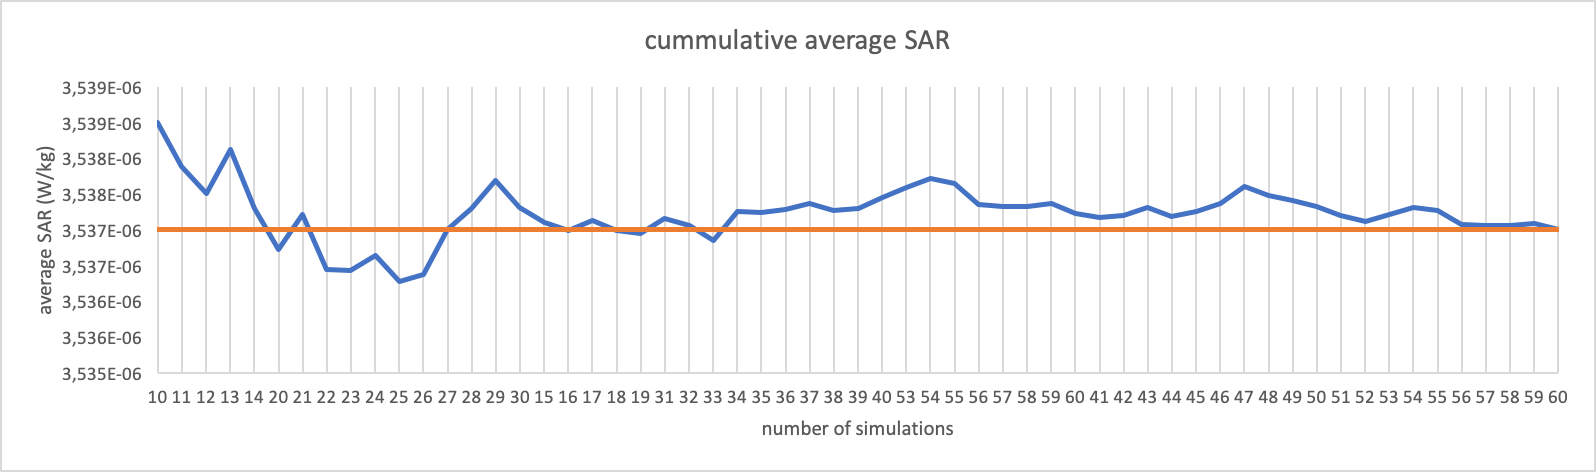
\includegraphics[width=\textwidth]{../results/numberOfSim/sarvssim.png}
  \caption{General design of a microstrip antenna}
  \label{fig:fhsar}
\end{figure}
\begin{figure}[th!]
  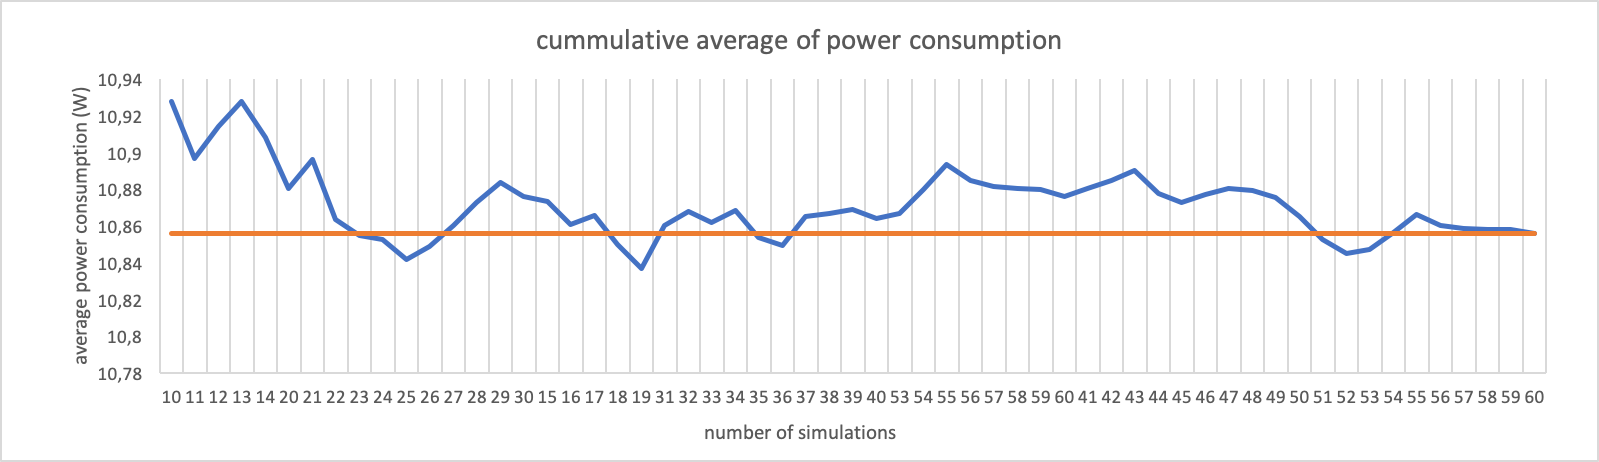
\includegraphics[width=\textwidth]{../results/numberOfSim/pcvssim.png}
  \caption{General design of a microstrip antenna}
  \label{fig:fhsar}
\end{figure}
\begin{figure}[th!]
  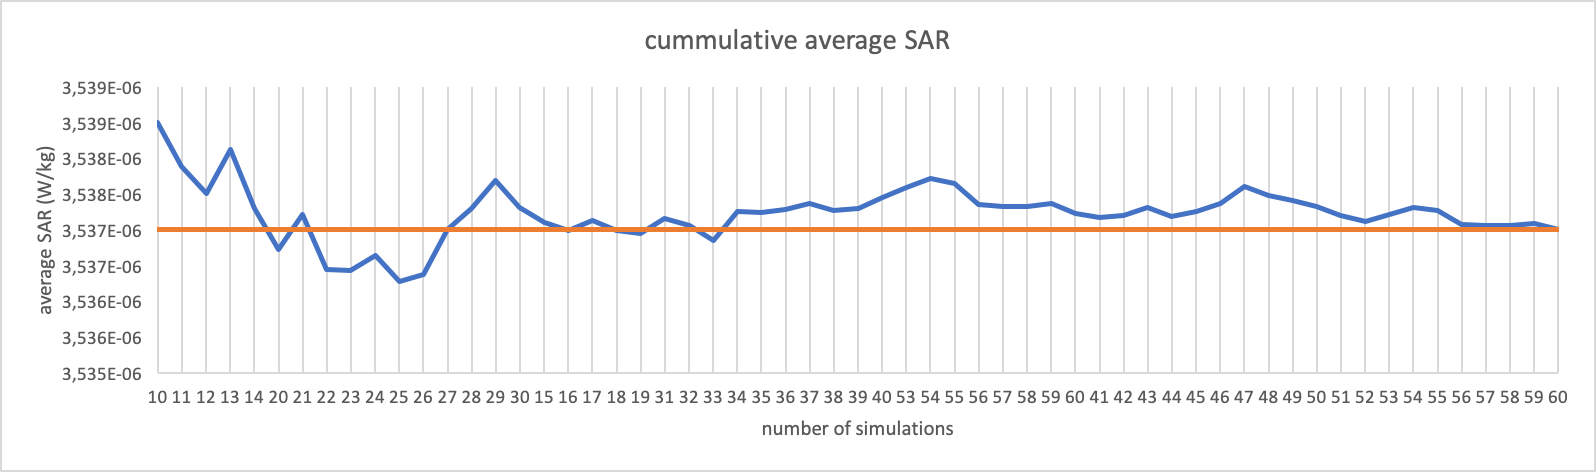
\includegraphics[width=\textwidth]{../results/numberOfSim/sarvssim.png}
  \caption{General design of a microstrip antenna}
  \label{fig:fhsar}
\end{figure}
\fi %remove to reanable section
%%%%%%%%%%%%%%%%%%%%%%%%%%%%%%%%%%%%%%%%%%%%%%%%%%%%%%%%%%%%%%%%%%%%%%%%%%%%%%%%%%%%%%%%%%%%%%%%%%%%%%%%%%%%%%%%%%%%%%%%%%%%%%%%%%%%
\section{Scenario 1: one user and one base station}

\subsection{The influence from the maximum transmission power}
\gls{LTE} makes usages of power control meaning that no more power will be used then strictly necessary. The actual 
transmit power $P_{tx}$ therefore ranges between 0 and the maximum input power. $P_{tx}$ is zero when either no user is 
present or the user is so far away that the actual transmit power would exceed the maximum transmission power.
Increasing the maximum transmission power won't influence the power consumption or $SAR_{10g}$ because the \gls{UABS} won't use more
then strictly required. It is therefore more useful to match the transmission power against a variable fly height. Figure \ref{fig:ptxfh}
shows a logarithmic  relationship showing that $P_{tx}$ increases fast at low altitude but slows down at lower altitudes. 

Figure \ref{fig:ptxfh} shows the minimal required energy by an \gls{isotropicradiator} in other to reach the user just below him.
As already discussed in \ref{sec:s1}, the user is outdoor and just below the \gls{UABS}. There is thus a free line-of-sight between both
radiators. It is clear that a step function is achieved from this. This is because multiple flying heights correspond to the same flying height.
When the flying height increases, so does the pathloss. \gls{LTE} tries to counteract this by increasing the power level. Each time 
the pathloss becomes to high, the power level of the antenna increases with one dBm. Doing so, decreases pathloss allowing the antenna to reach
the user again. When the flying height immediately after increases again, the pathloss also increases but not enough to force the drone to 
increase his power level again. This explains the discontinue step function. If the tool would make usage of smaller step size, a more continuous 
logarithmic function would be achieve. This would however worsen the time complexity because increasing the power level to exceed the pathloss
 happens in smaller steps. The red line indicates the default maximum transmission power used during simulations. 
In a free line-of-sight scenario with only one user, a \gls{UABS} can fly up to 387 meters before losing connection.

This scenario is investigated with a microstrip patch antenna using power consumption optimization. However, these parameters does not matter.
While an \gls{isotropicradiator} no attenuation, a microstrip patch antenna does but since the user positioend in the perfect center of the main beam there
won't be any attenuation in eighter cases. Also the optimization wont' make a difference. The goal of the  strategy is to decide wich drone is most suitable for which
users. Since there is only one user and one possible position for the drone, both optimization strategies behave identical.

\begin{figure}[h!]
  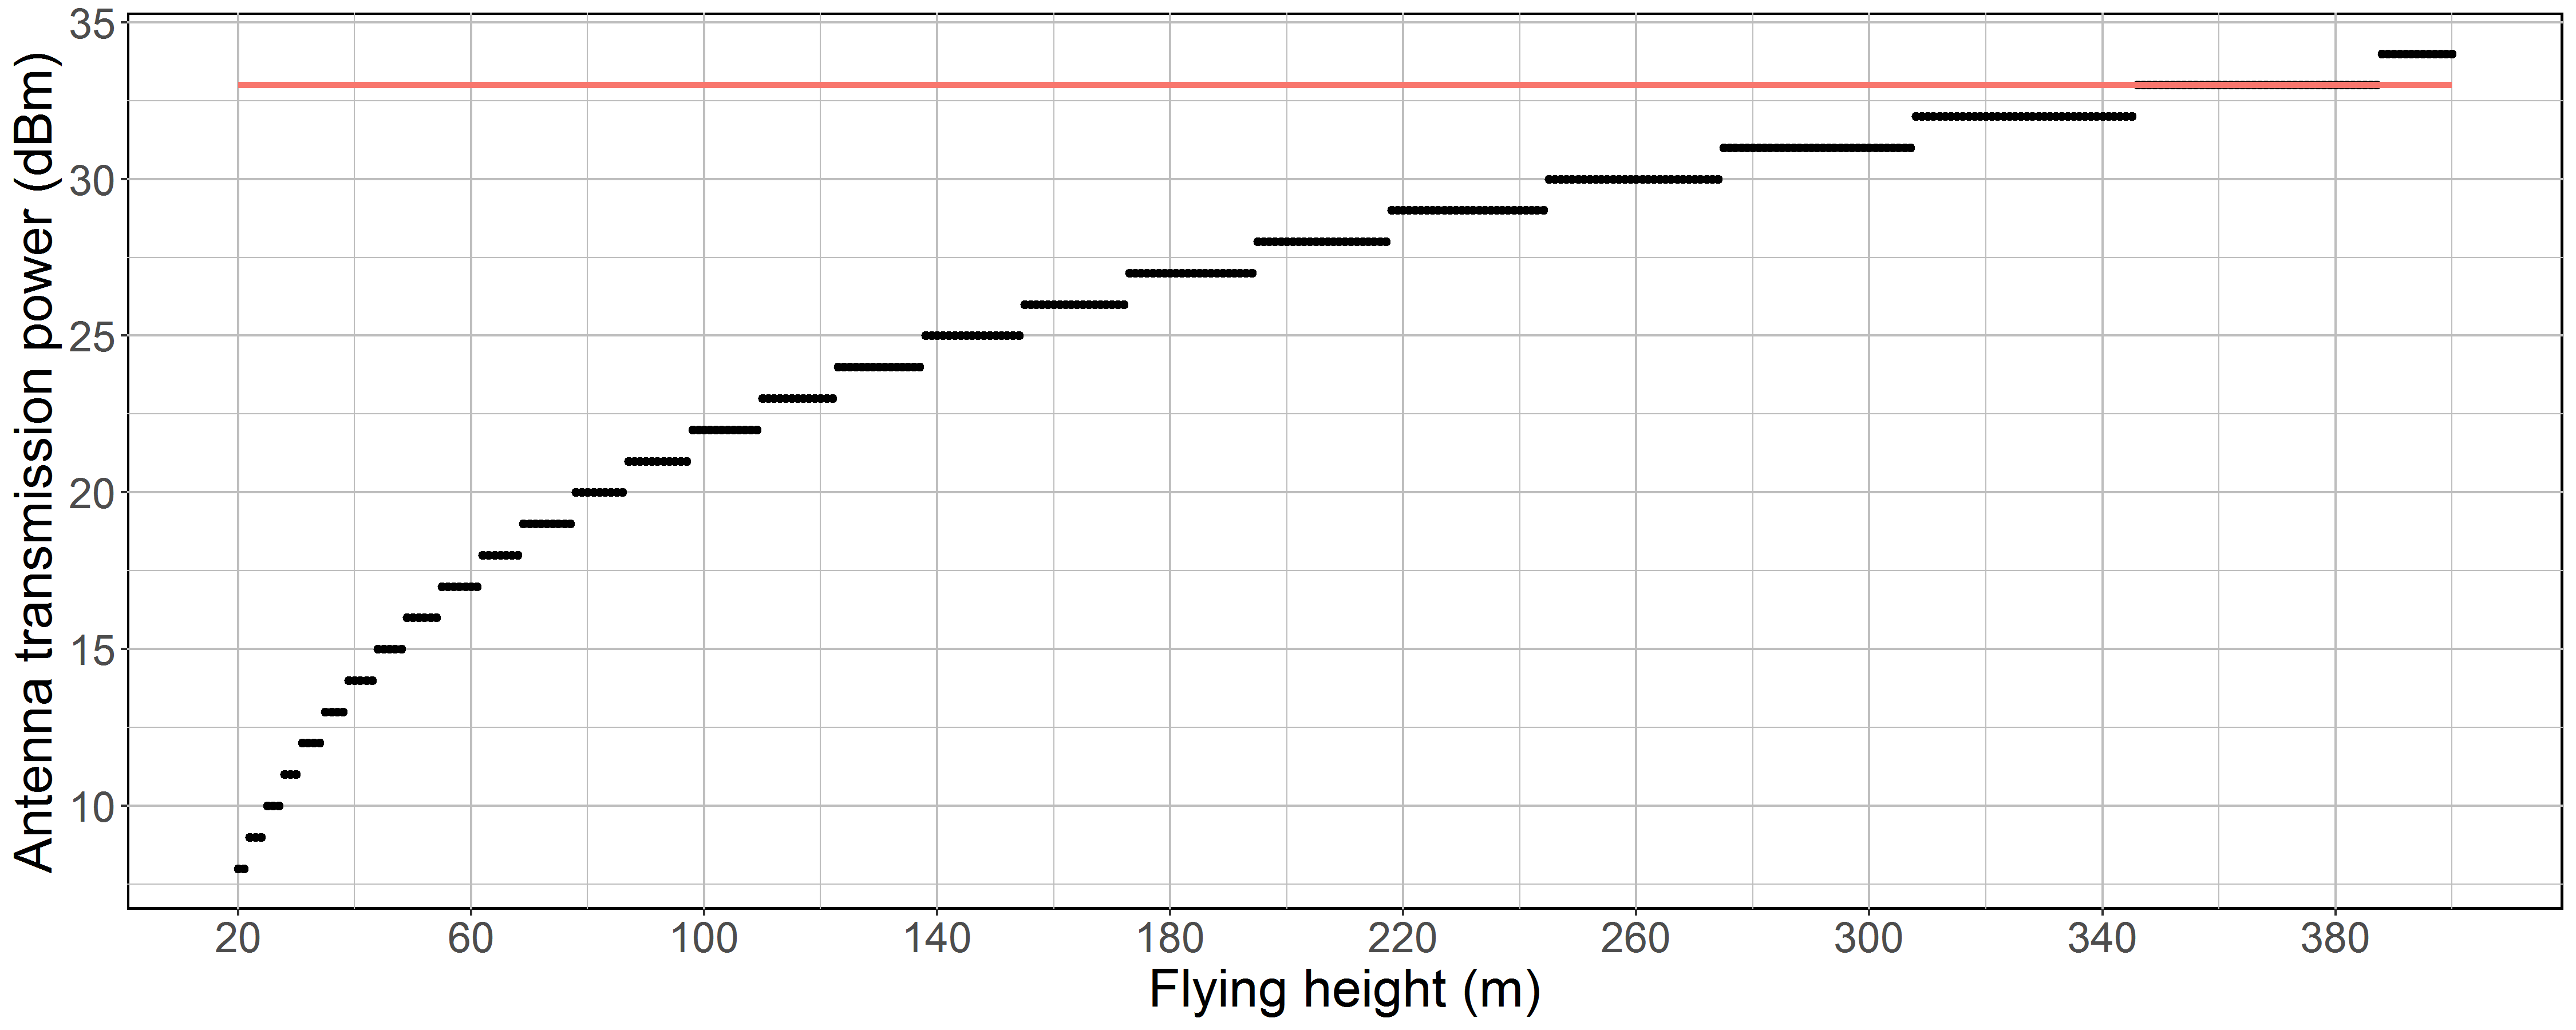
\includegraphics[width=\textwidth]{../results/s1/ptx.png}
  \caption{Minimal required transmission power by the antenna to reach the ground just below him.}
  \label{fig:ptxfh}
\end{figure}

\subsection{Influence of the flying height}
\label{sub:senario1_influenceOfFlyHeight}

This section investigates how the fly height of the \gls{UABS} influence $SAR_{10g}$ and power consumption. In figure \ref{fig:fhsar}
becomes clear that with an increasing flying height, the specific absorption rate grows exponentially 
which is also the case for the power consumption (fig. \ref{fig:pcsar})  

Figure \ref{fig:s1_fhsar} shows the induced electromagnetic radiation for our user. The red line shows the $SAR^{own device}_{10g}$. This radiation very low when the \gls{UABS}
is close to the ground but increases exponentially at higher flying altitudes. The green line represent the $SAR^{basestation}_{10g}$ which shows the same discontinue 
behavior from in figure \ref{fig:ptxfh}. As explained before, \gls{LTE} makes usage of power control. Meaning that the power transmission only increases when pahtloss 
increases up to the point where the power level exceeds its maximum after which connection is lost completely and exposure drops to zero. 
This behavour causes the electromagnetic radiation experienced by the user to be almost constant. The slightly visible variation is just an extention of the reason 
why figure \ref{fig:ptxfh} forms a step function. When the power level increases with $1 dBm$, it is more then strictly required causing the electromagnetic radiation to 
slightly increase. Just before an energy jump, pathloss and power level are perfectly balanced generating the lowest possible electromagnetic radiation possible.

Figure \ref{fig:s1_fhsar} doesn't show radiation from neighbours, because there are non present in this scenario. Finally, all these values are added as explained in formula
\ref{eq:overallSARwb}. 

The figure shows that for low flying drones, \gls{UABS}s are the main source of electromagnetic radiation.
This changes around 80 meters where \gls{UL} electromagnetic radiation of the \gls{UE}
exceeds \gls{DL} radiation in order to still be able to reach the high flying \gls{UABS}s.


\begin{figure}[th!]
  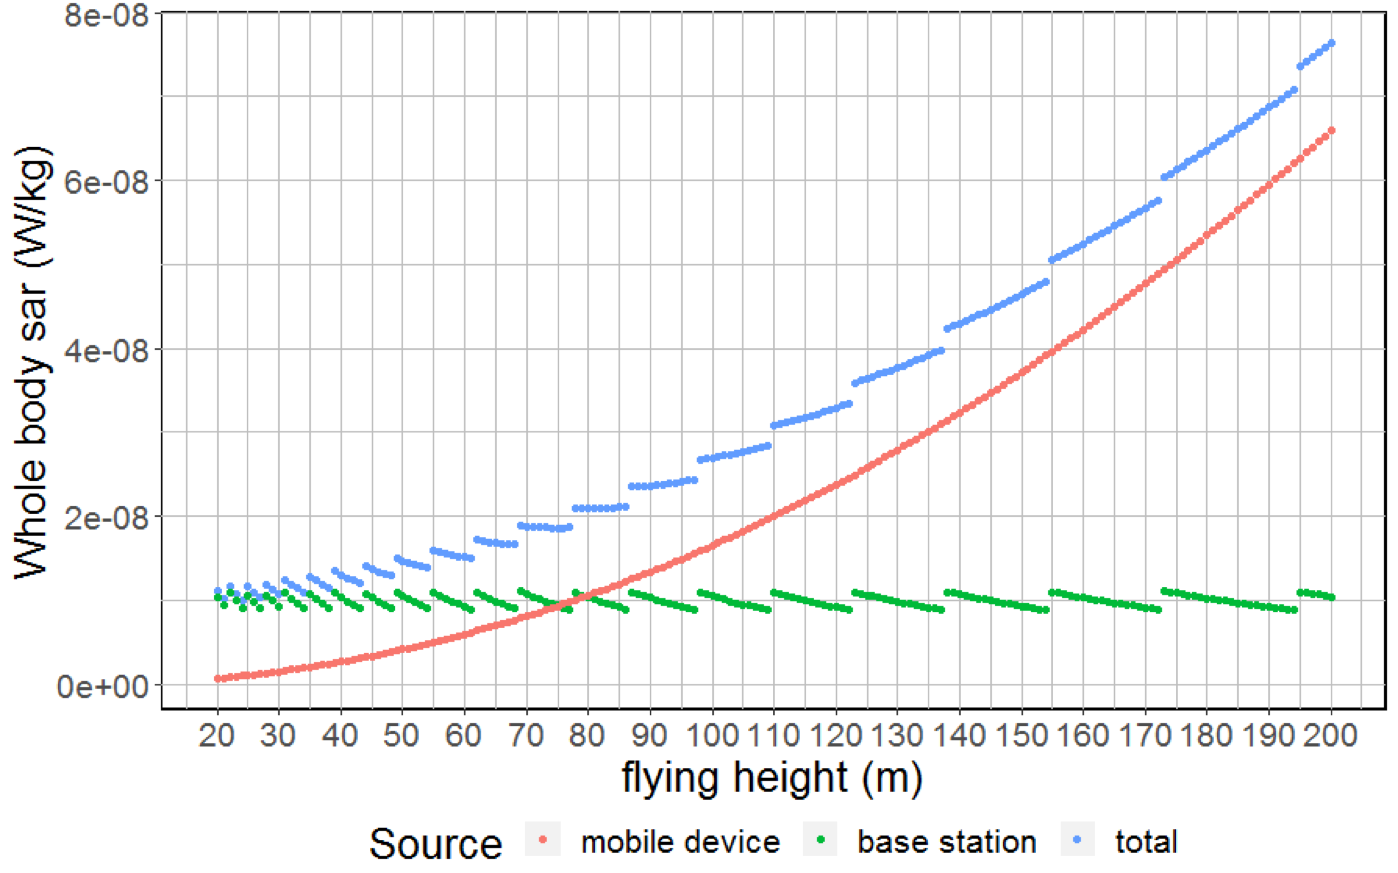
\includegraphics[width=\textwidth]{../results/s1/fhvssar2.png}
  \caption{General design of a microstrip antenna}
  \label{fig:s1_fhsar}
\end{figure}

%%%%%%%%%%%%%%%%%%%%%%%%%%%%%%%%%%%%%%%%%%%%%%%%%%%%%%%%%%%%%%%%%%%%%%%%%%%%%%%%%%%%%%%%%%%%%%%%%%%%%%%%%%%%%
\section{Scenario 2: increased traffic}

\subsection{Influence of the flight altitude}
This scenario investigates how the network consisting of one \gls{UABS} behaves when applied on an ordinary day during rush hour. 
On average, 224 active users are distributed uniformly over the city center of Ghent. 
Chart \ref{fig:s2fhvsdl} shows how the downlink exposure is influenced by flying height of the \gls{UABS}. 
Increasing the flying height has a direct influence on the total downlink exposure of an individual user. 
This is because if a drone flies higher, there is less penetration loss from obstructing buildings.

A power consumption optimized network with an \gls{EIRP} antenna (yellow) has the highest exposure. 
This is logical when comparing with an EIRP antenna in an exposure optimized network (red). 
However, when looking at chart \ref{fig:s2fhvspc}, the power consumption in a power consumption optimized network is worse 
than in an exposure optimized network. To understand this, the behavior of the deployment tool needs to be understood first. 
We know that a power consumption optimized network will result in few high powered \gls{UABS}s while an exposure optimized network 
generates a lot of low powered \gls{UABS}s. When only limited amount of \gls{UABS}s are available, 
like only one in this scenario, the tool will only keep \gls{UABS}s which cover most of the users. 
Therefore, is the power consumption in a power consumption optimized network way higher. 

\begin{figure}[h!]
  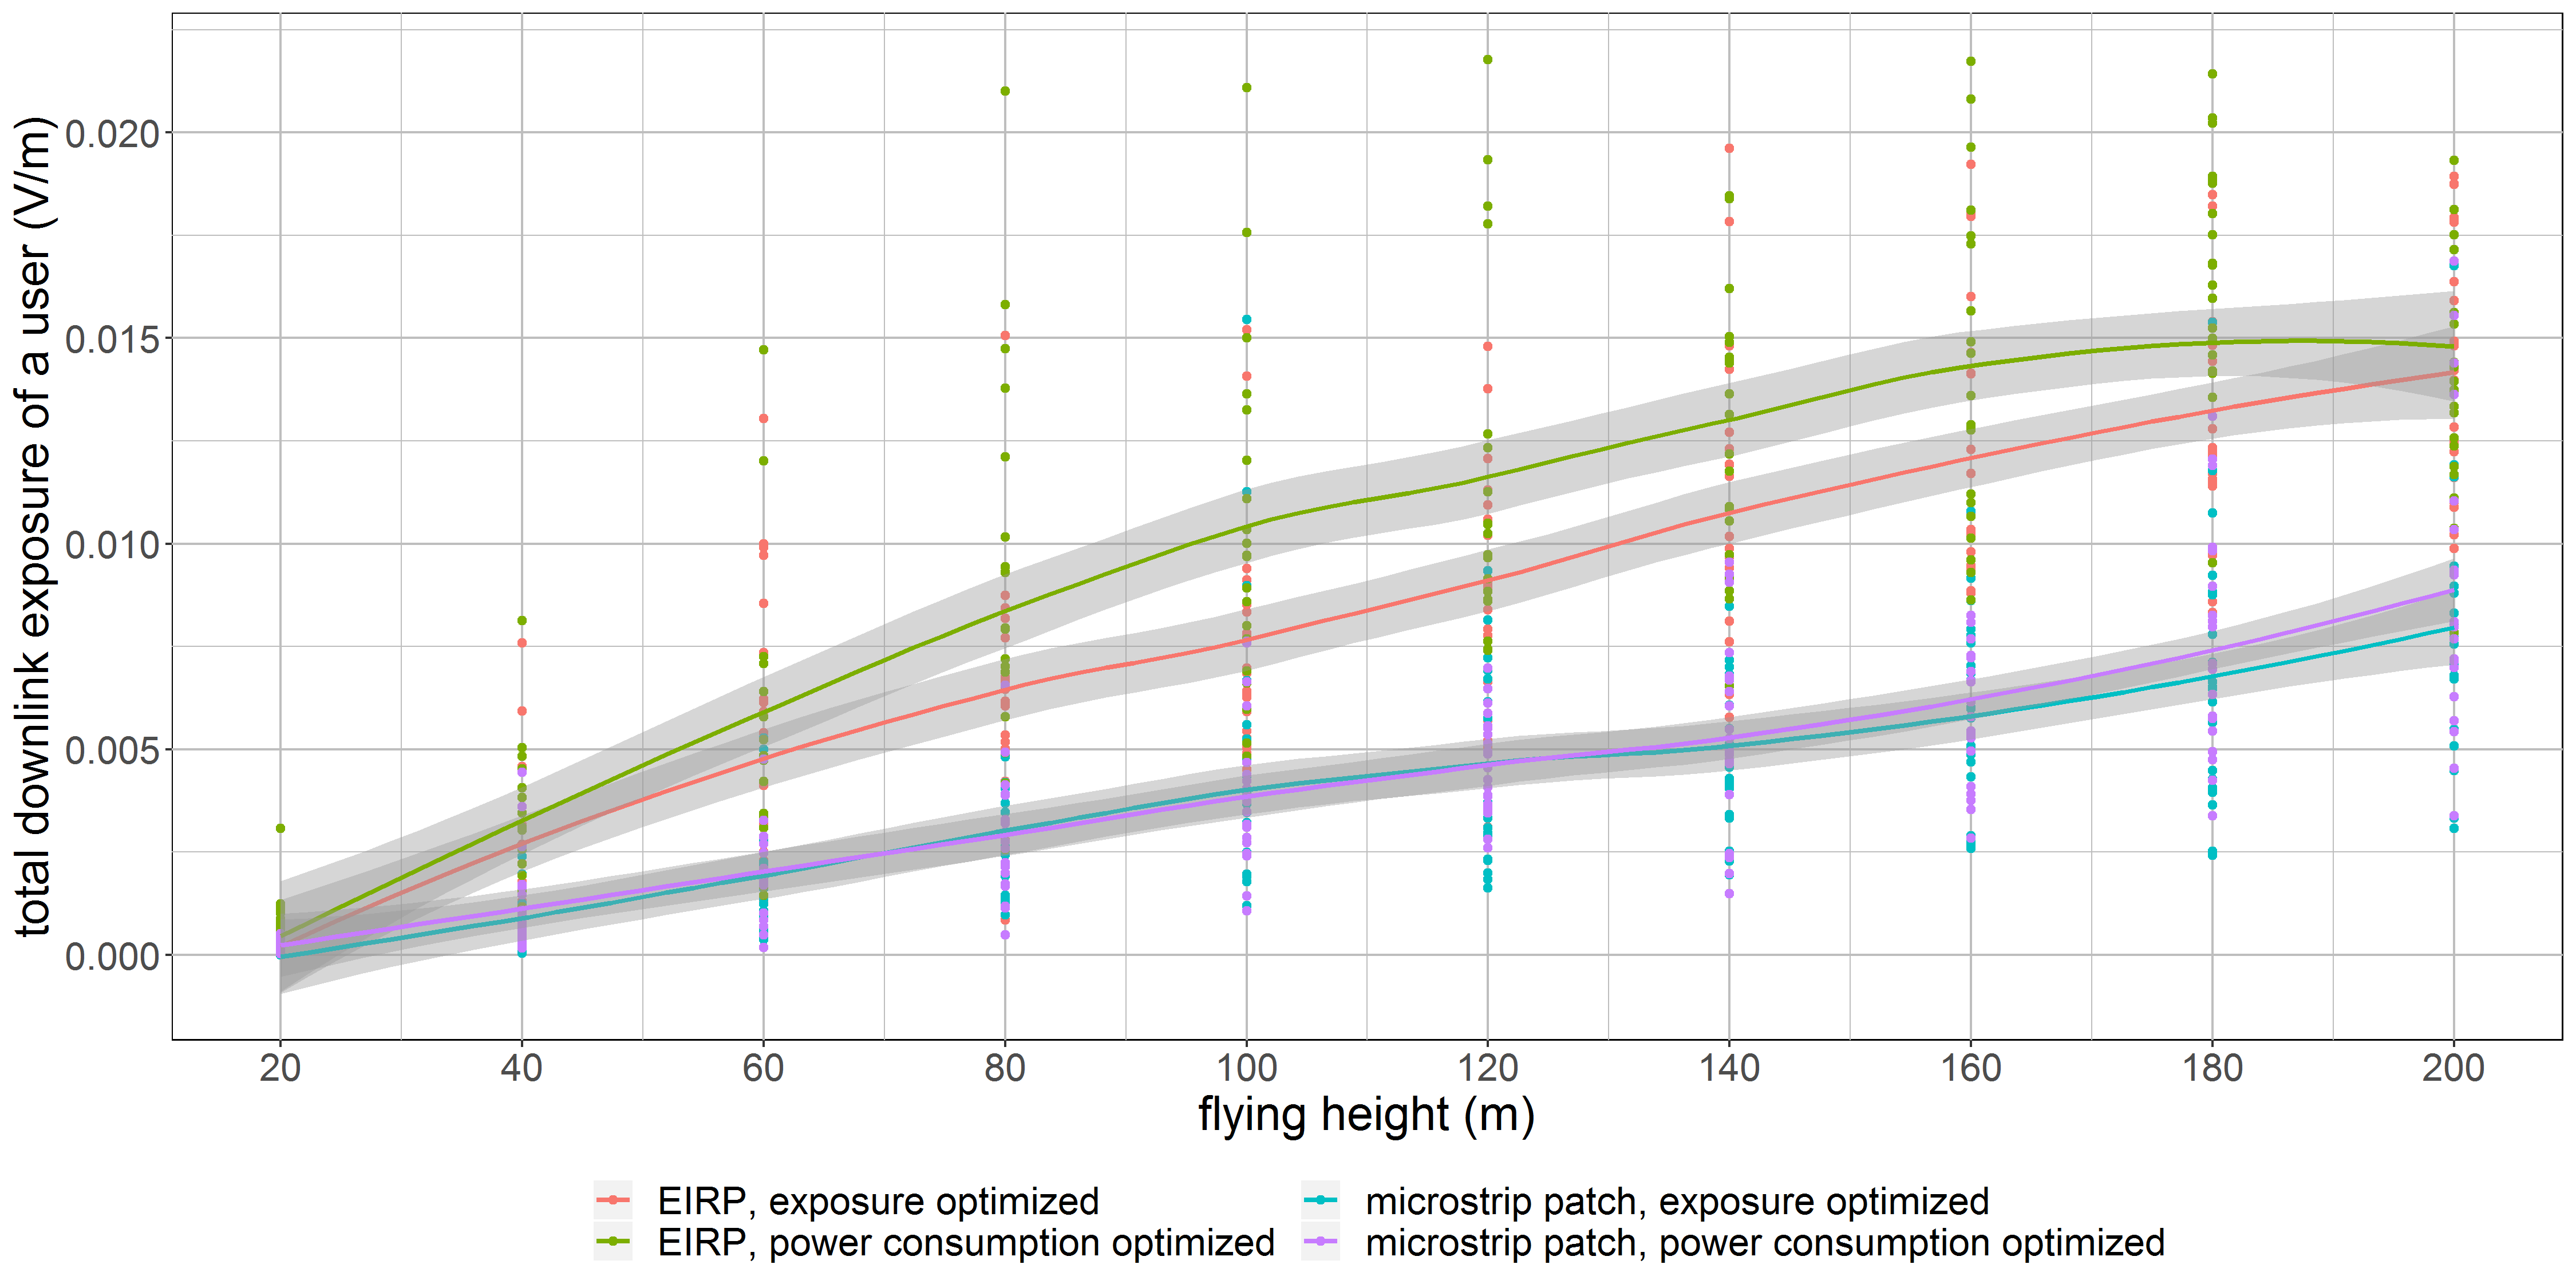
\includegraphics[width=\textwidth]{../results/s2/fhvsdl.png}
  \caption{The influence of the flying height on the weighted average downlink exposure of users in the network.}
  \label{fig:s2fhvsdl}
\end{figure}

\begin{figure}[bh!]
  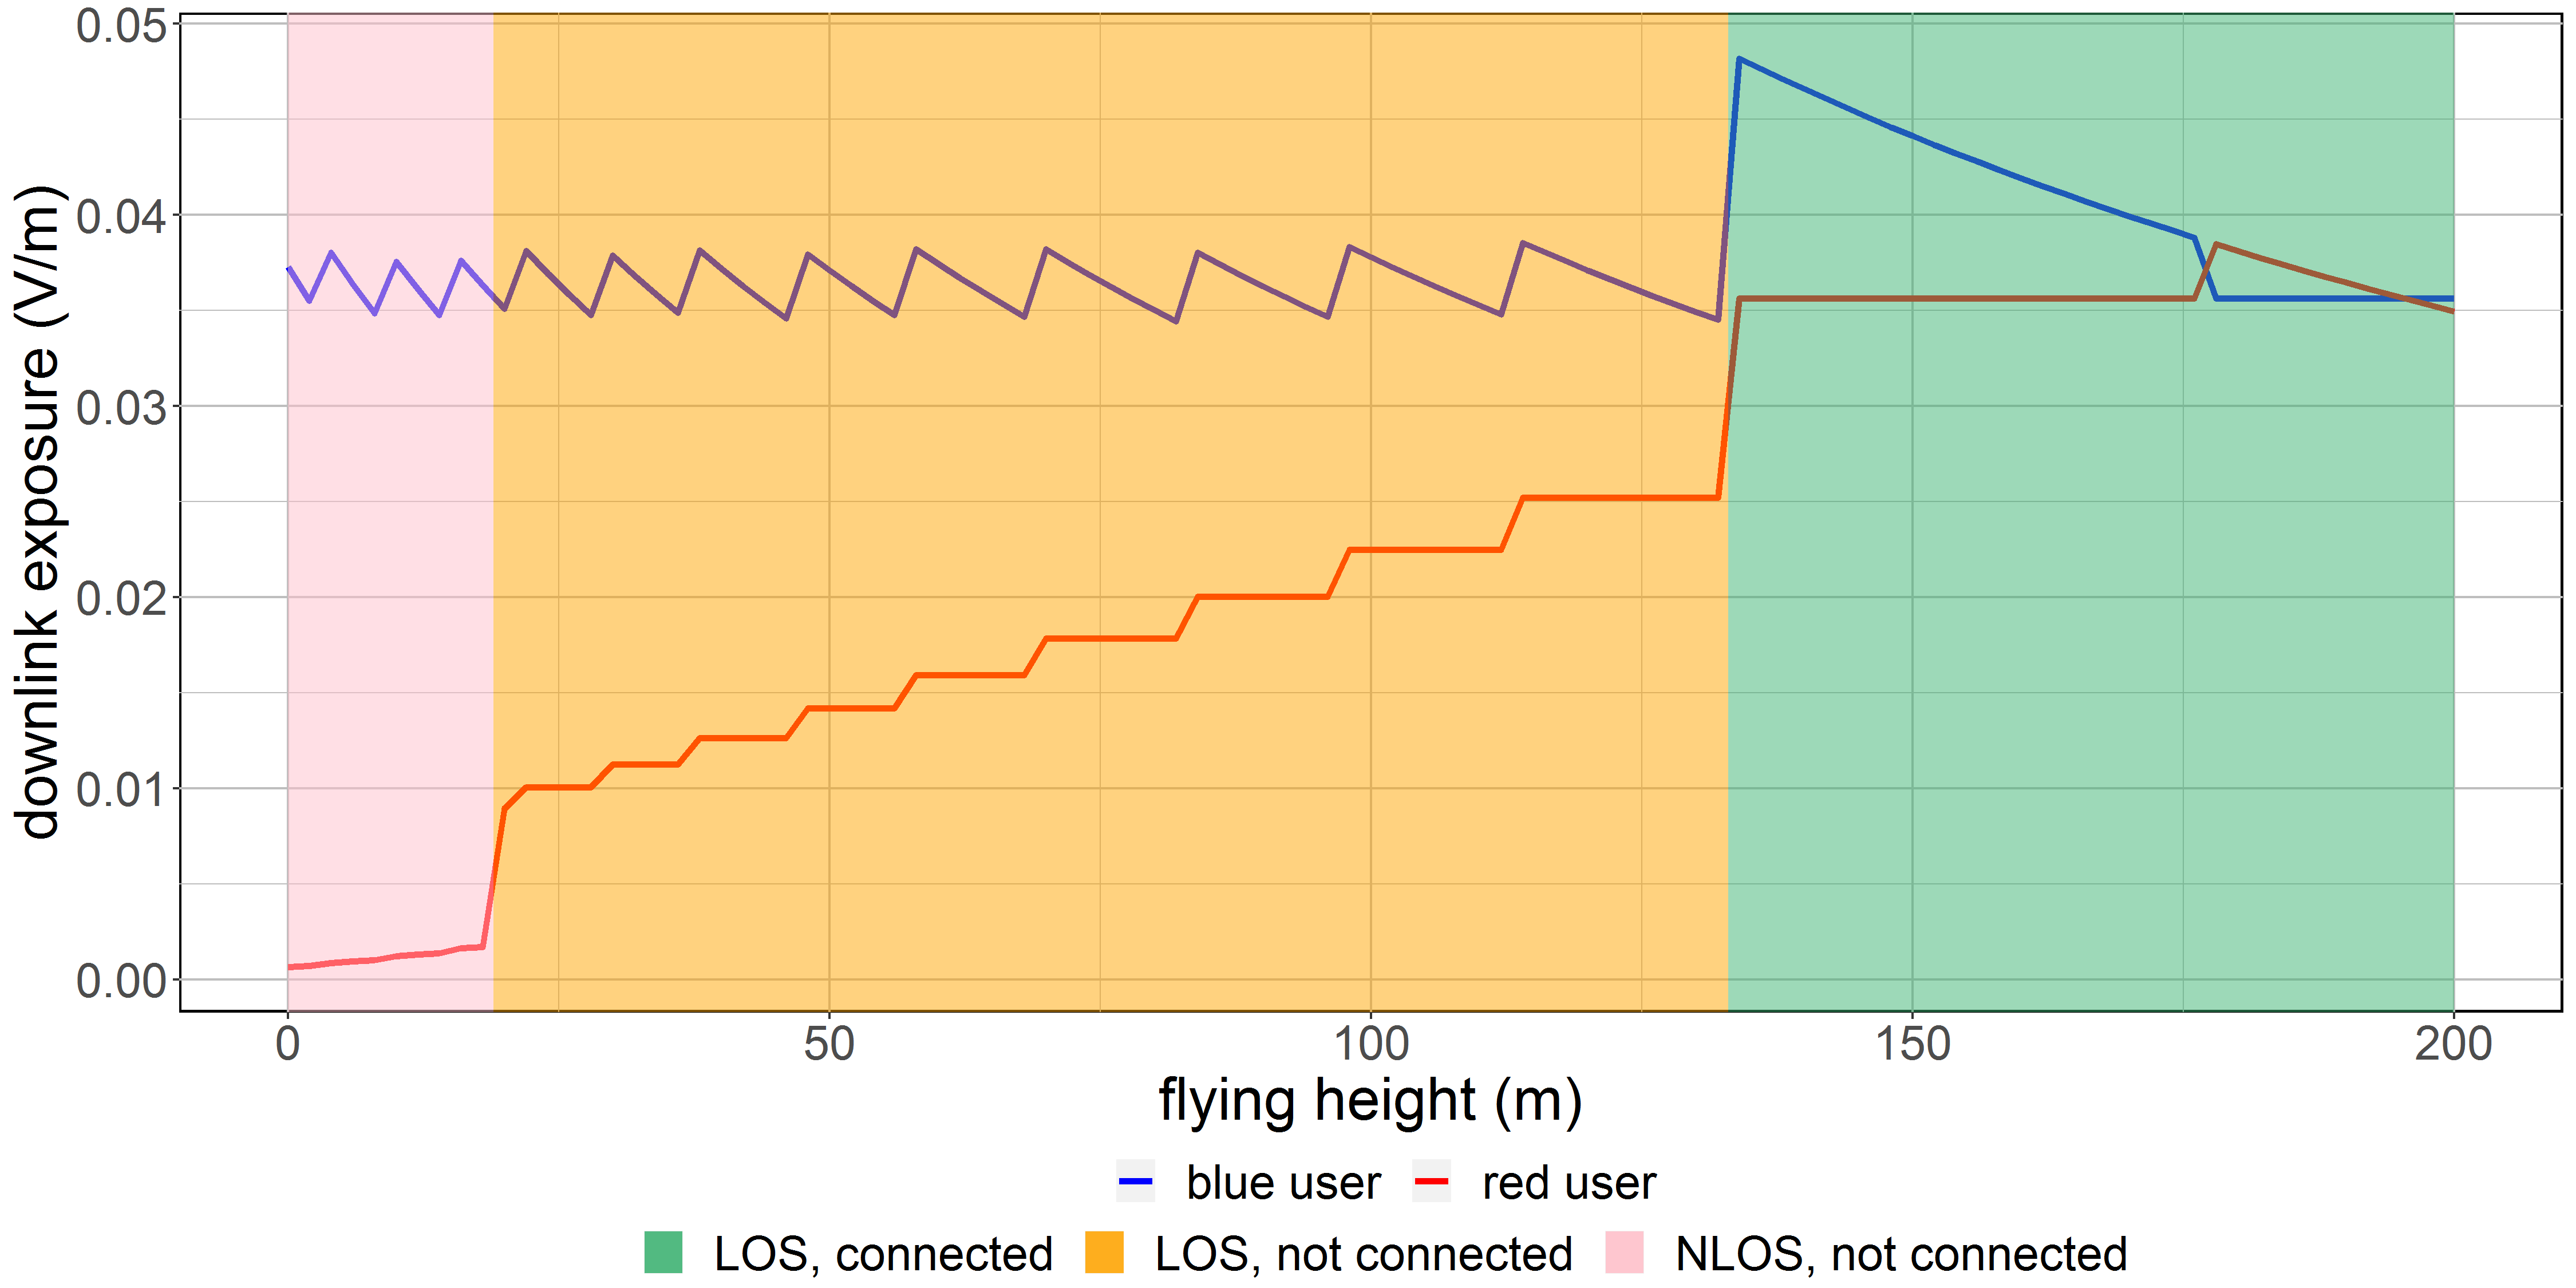
\includegraphics[width=\textwidth]{../results/s1/prove.png}
  \caption{Scenario 2 with only 2 users}
  \label{fig:pcsar}
\end{figure}

TODO: tekening van twee gebruikes met drone

To prove the correctness of figure \ref{fig:s2fhvsdl}, the scenario has been investigated for two users called the red and blue user who 
are 90 metres separated from each other. The path between both is obstructed by a building.
Scenario 1 already explained that the charts can be simplified and the blue line is in fact constant between the zero and 130 metres.
The chart shows thus that the \gls{UABS} is positioned above the blue user. The orange user is in \gls{NLOS} as long as the \gls{UABS} remains below 20 metres.

Once the \gls{UABS} increases, the user becomes into \gls{LOS} but still remains uncovered. This is because the tool initally locate a possible 
\gls{UABS} above each user and thereafter performs a  fitness function. The applied fitness function must have decided that it is better to connect 
each user to the \gls{UABS} above him. At a final state, the tool check whether the number of online drones does not exceed the capacity of the facilityCapacity
which is here the case. The tool therefore deactivates one \gls{UABS} causing the orange user to be uncovered. One could argue that the 
the orange user should be connected to the online drone who is only 90 metres away. This would however require the online drone to increase his power consumption which 
would make the decisions made by the optimization strategy obsolete.

When a drone flies higher, the difference in distance between both users and the base station decreases. In other words, the Pythagorean theorem shows that when the flying height of the 
\gls{UABS} increases, the distance with the blue user increases faster compared to the distance between that same \gls{UABS} and the orange user.

At 130 metres, the tool decides to connect both users to the same UABS. Therefore, it increases it's power consumption so the orange user would  have the minimal 
required electromagnetic exposure. This has of course a negative influence for the blue user who is way closer and experience a much higher exposure level.

Around 180 metres, the  orange and blue line switch. This is because the drone switches position. As explained before, the tool assignes two possible drones, one above 
each user. The tool must have decided that connecting both users to the other drones improves the fitness function of the entire network even though that difference might be 
very little.



\begin{figure}[h!]
  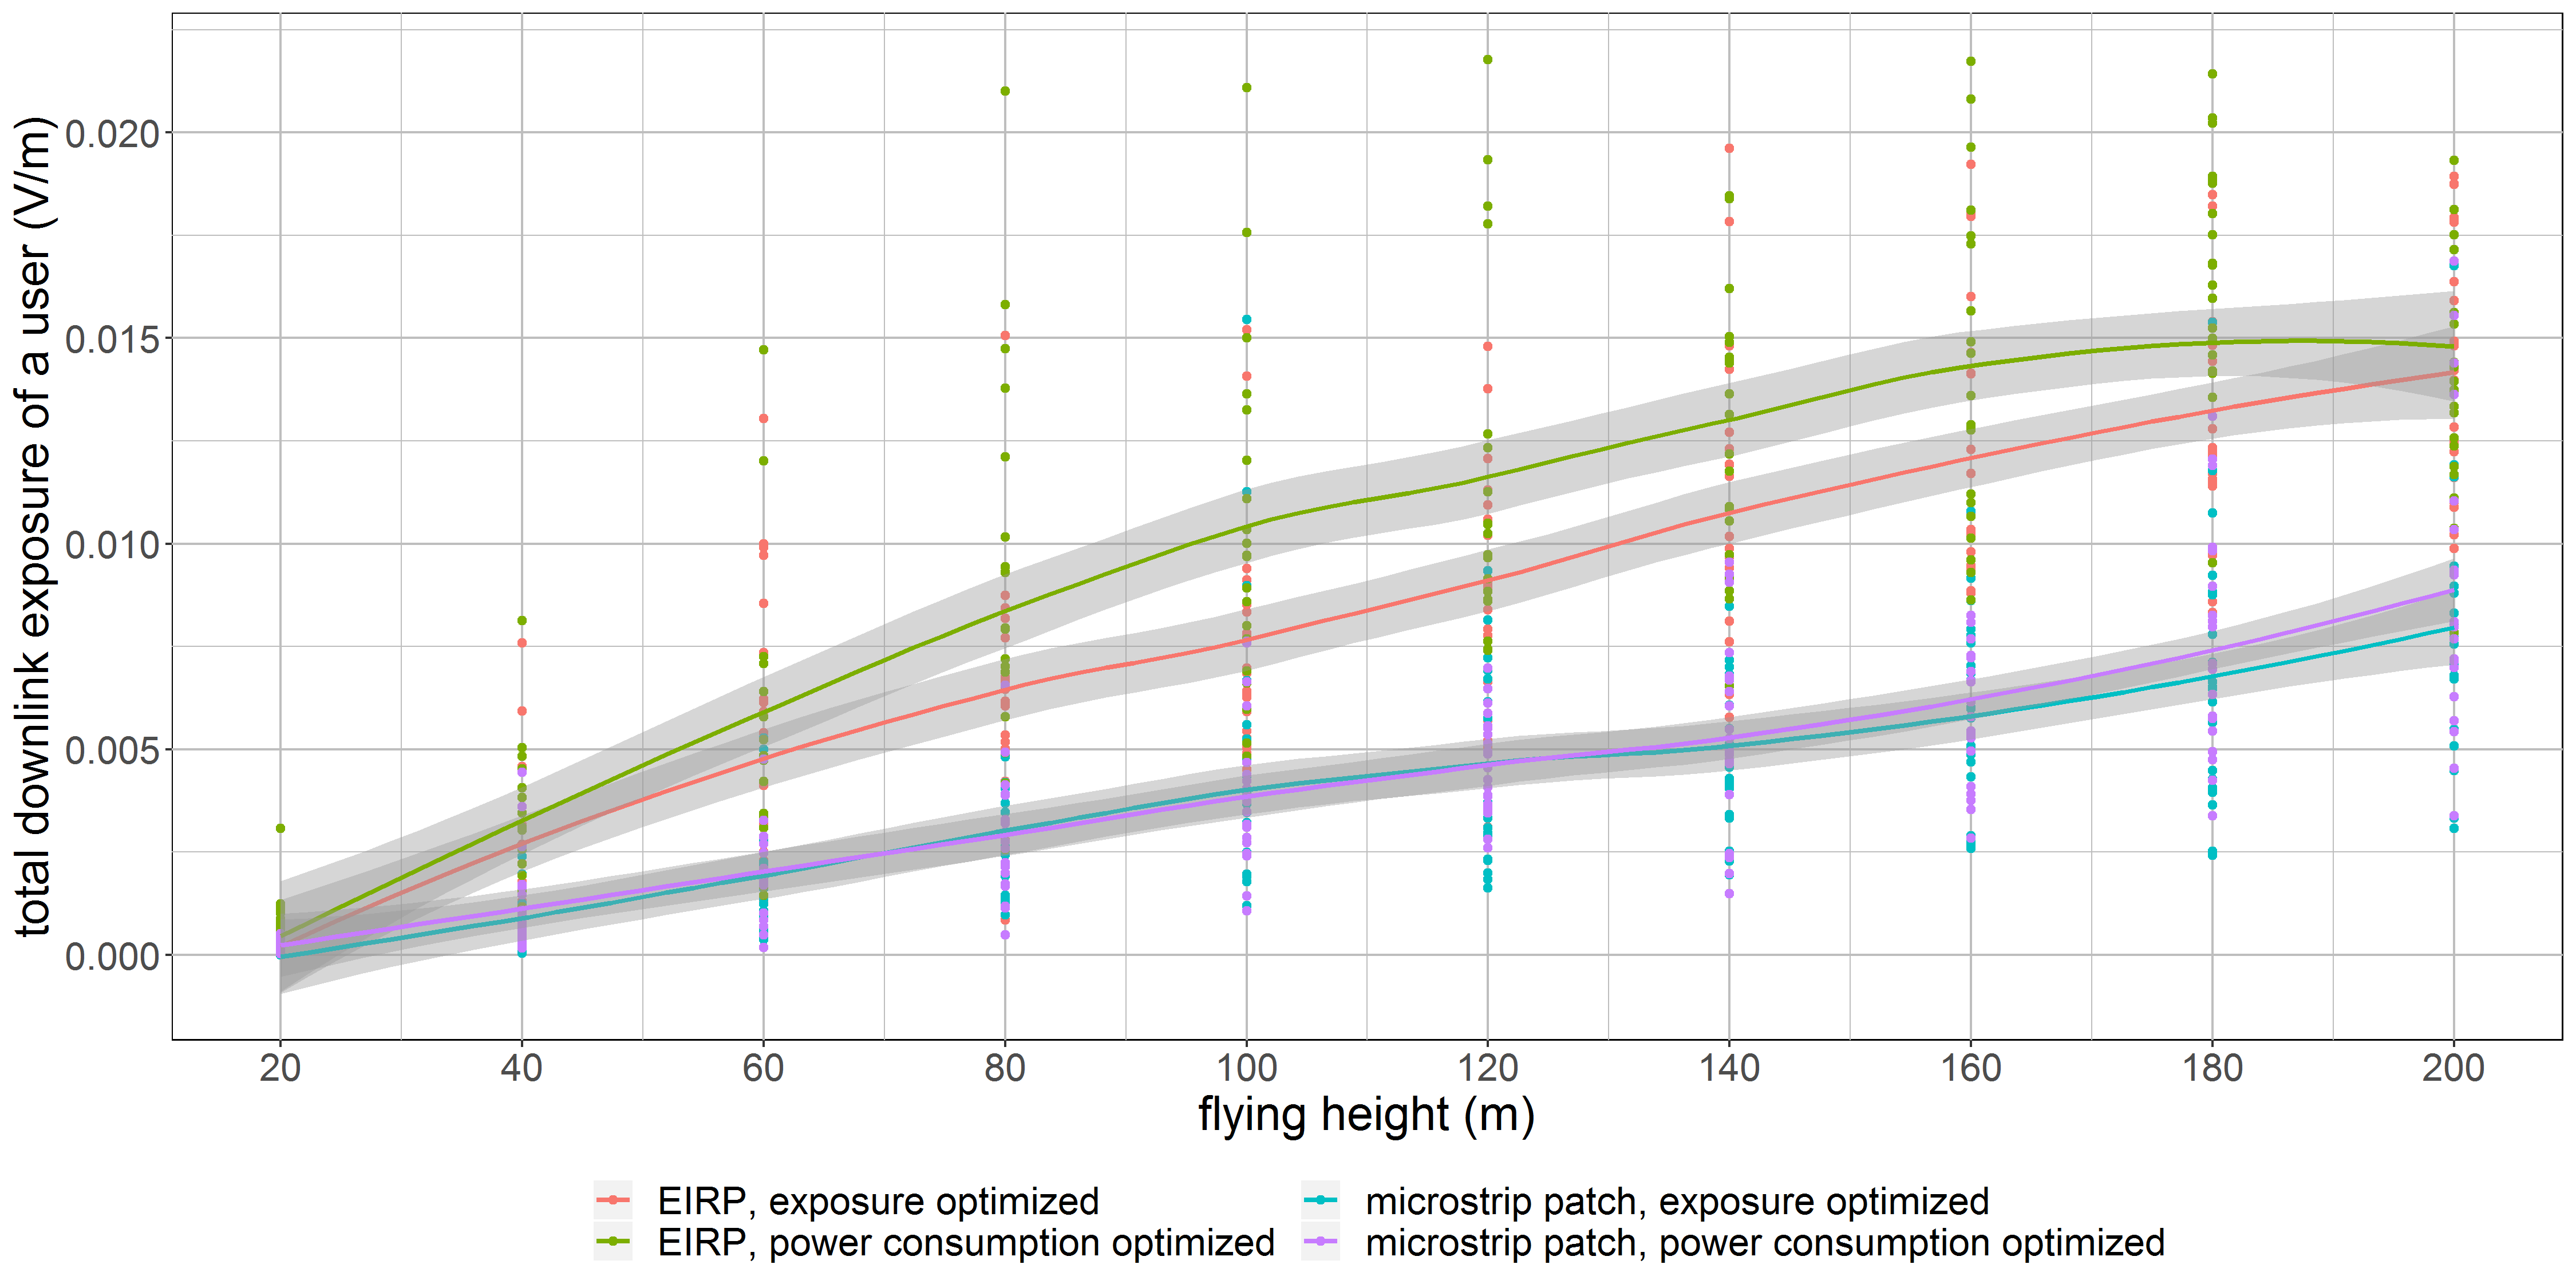
\includegraphics[width=\textwidth]{../results/s2/fhvsdl.png}
  \caption{The influence of the flying height on the total power consumption of the network.}
  \label{fig:s2fhvspc}
\end{figure}


Chart  \ref{fig:s2fhvscov} shows that the flying height has a positive influence on the user coverage. 
When a \gls{UABS} flies higher, there is less pathloss between the user and the drone caused by buildings. 
As mentioned before, a power consumption optimized network will result in few high powered \gls{UABS}s. 
The tool removes all \gls{UABS}s except the one with most users. 
The network therefore exist out of one high powered \gls{UABS} compared to the exposure optimized network with one drone which 
will be less powered. Since yellow has a higher power level, also more users will be covered.

When replacing the fictional \gls{EIRP} antenna with a microstrip patch antenna, the percentage of covered users drops for both 
optimization strategies. This is because users who have a higher horizontal distance between themselves and the \gls{UABS}, 
experience a higher attenuation. Also, when a microstrip patch antenna is positioned higher, the range of the antenna increases 
since the angle between the user and the \gls{UABS}s main lob decreases. The user will therefore experience less attenuation.

It becomes also clear that this advantage is limited. For a scenario of 224 users and one drone, the user coverage won’t increase
 significantly anymore around an altitude of 120m.

\begin{figure}[h!]
  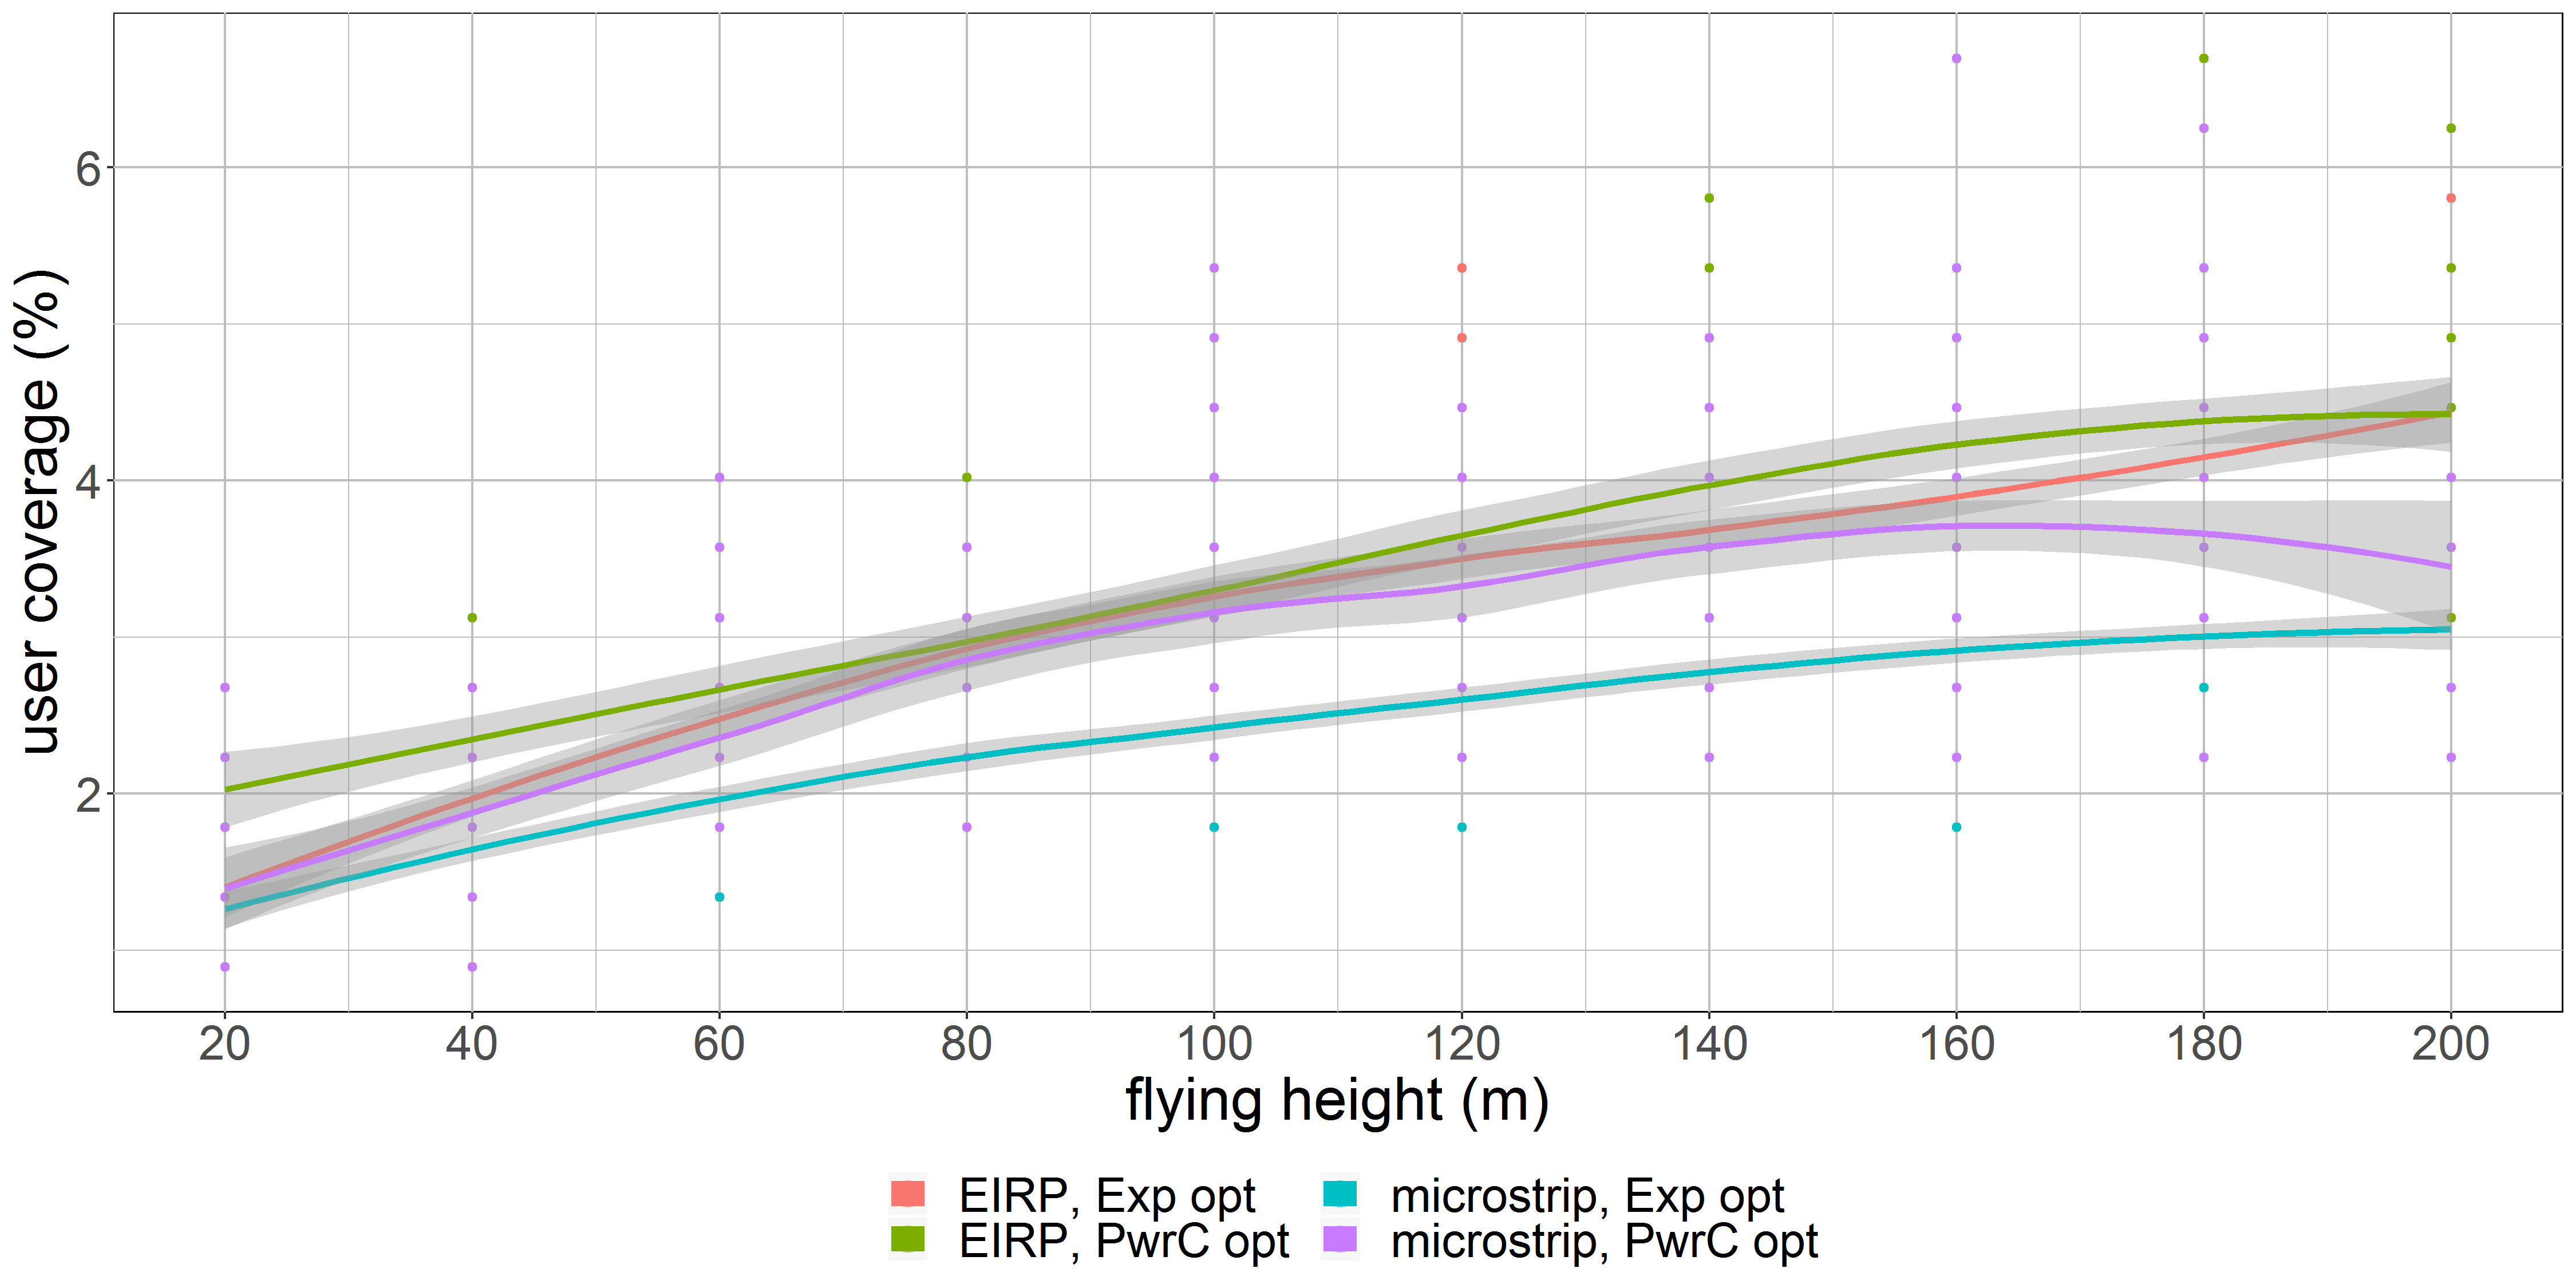
\includegraphics[width=\textwidth]{../results/s2/fhvscov.png}
  \caption{This graph shows the percentage of covered users by one drone for different flying heights.}
  \label{fig:s2fhvscov}
\end{figure}

Chart \ref{fig:s2fhvssar} shows the whole body SAR10g, deducted from all electromagnetic sources. This being exposure of all \gls{UABS}s,
 the uplink exposure from the user’s own device and the exposure of the devices from all other users. 
 Thereafter, the weighted average of all whole body SAR10g values in the network is calculated with the 50th and 95th percentile 
 being the most important values. This is because not only the mean values are important but also users who experience higher 
 levels of whole body SAR10g.


\begin{figure}[h!]
  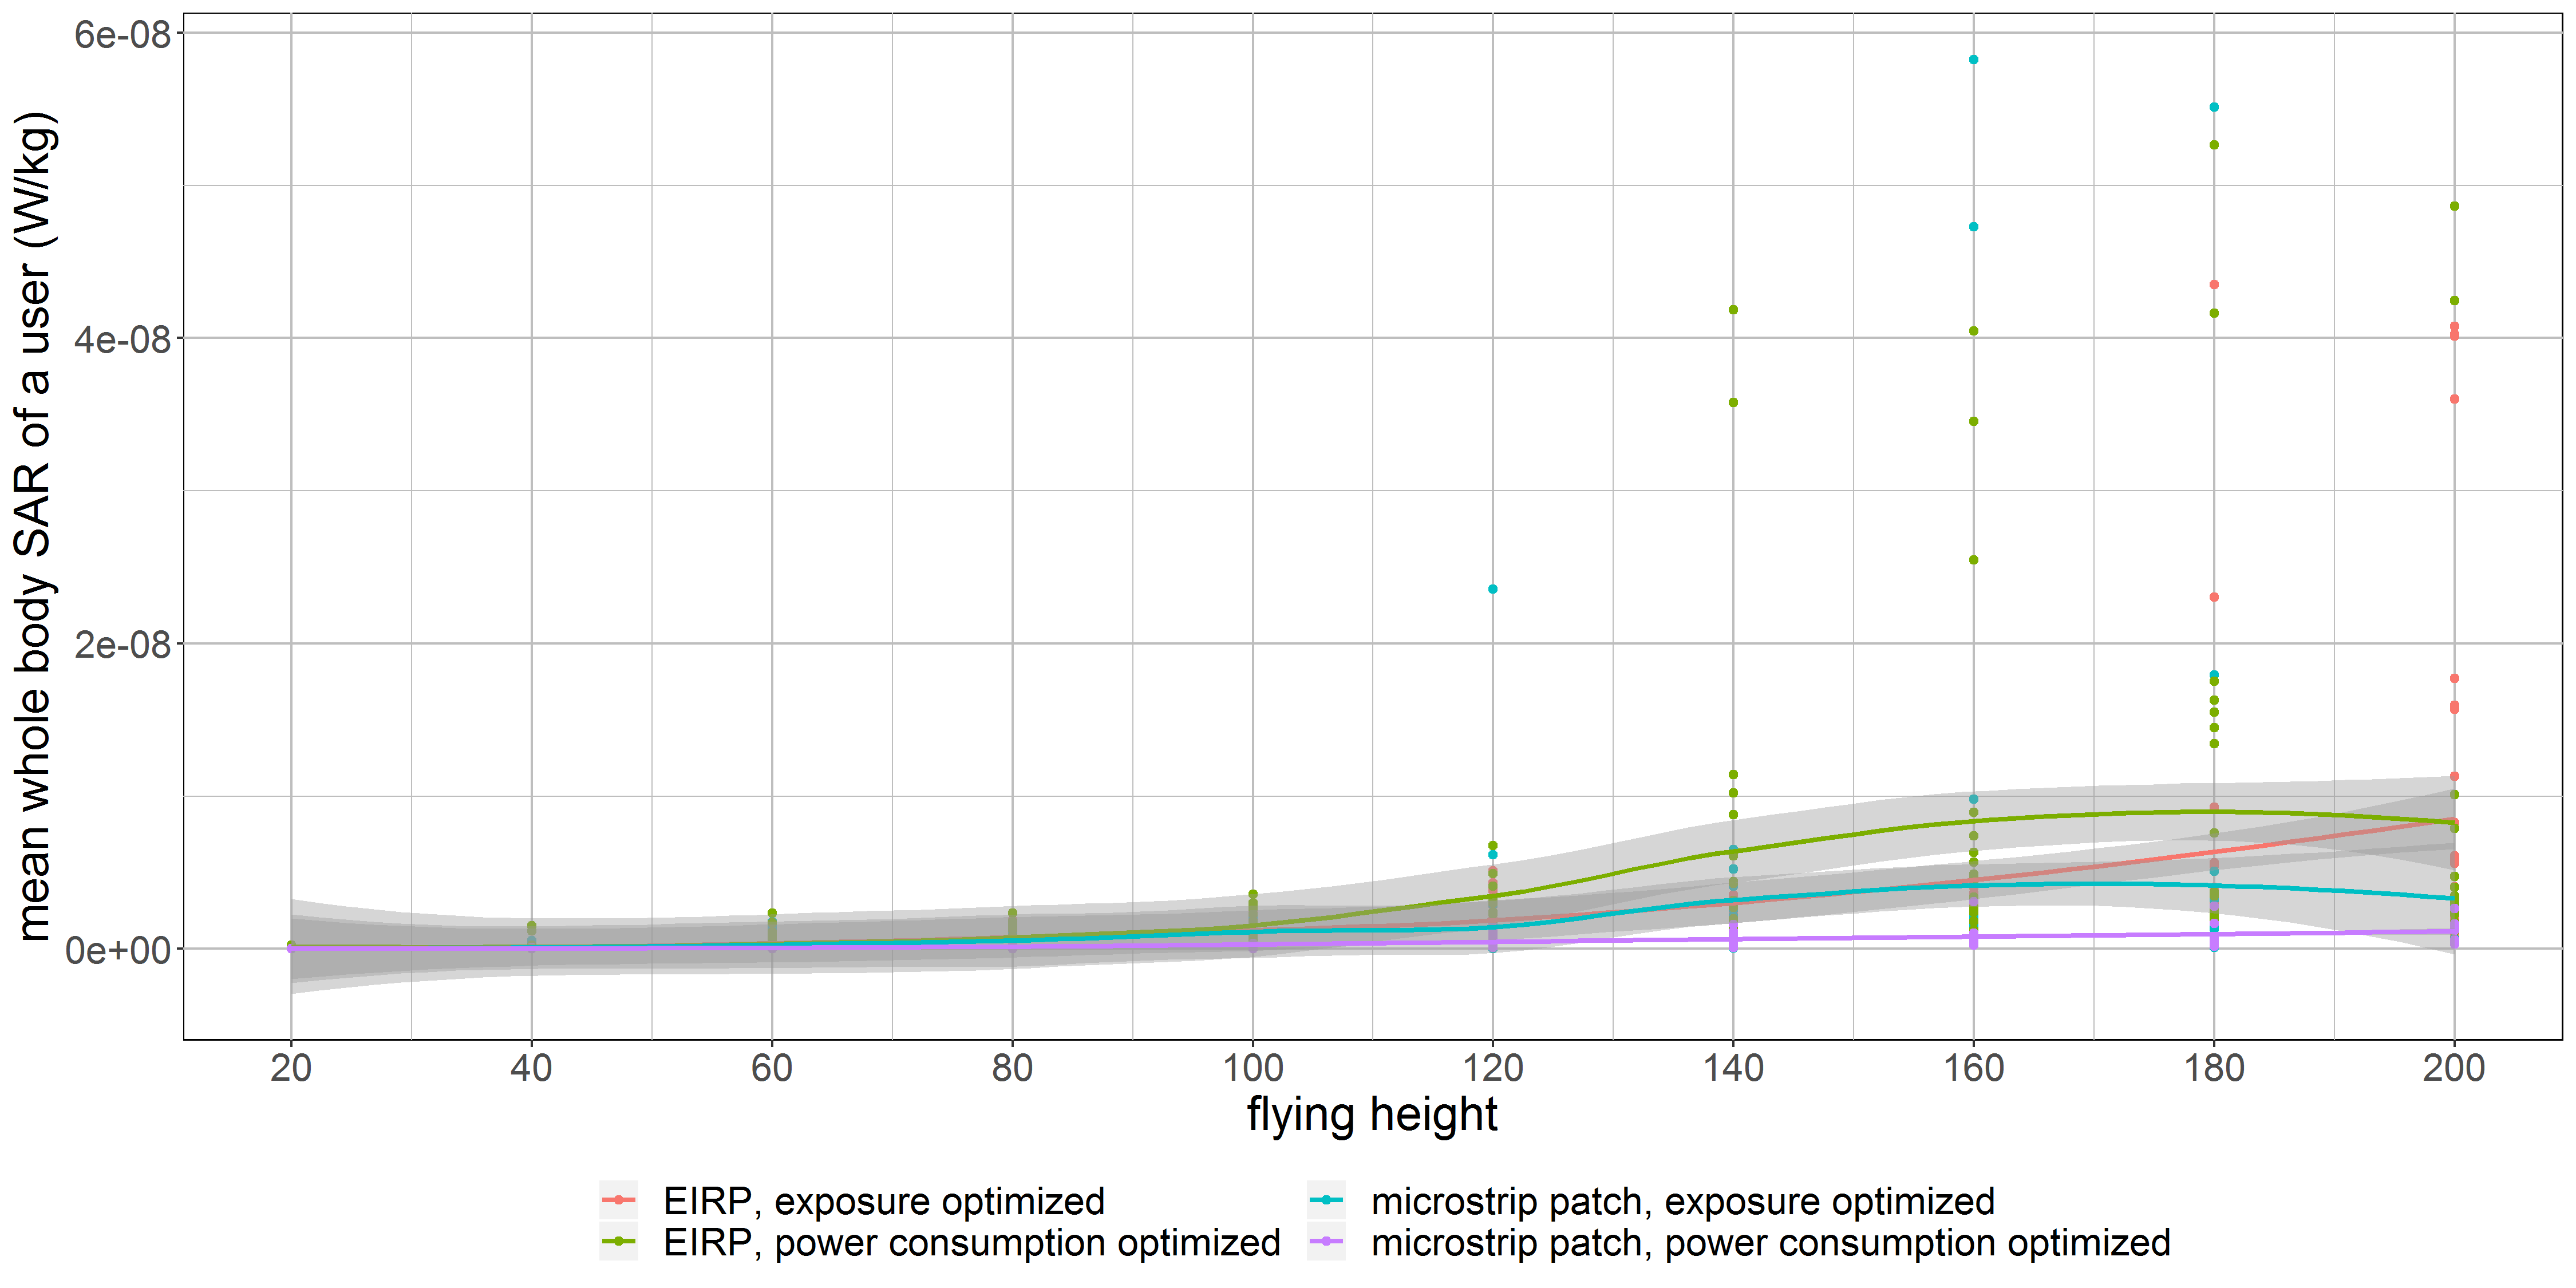
\includegraphics[width=\textwidth]{../results/s2/fhvssar.png}
  \caption{The influence of the flying height on the weighted average $SAR_{10g}$ of users in the network.}
  \label{fig:s2fhvssar}
\end{figure}


\subsection{Influence of the number of users}


%%%%%%%%%%%%%%%%%%%%%%%%%%%%%%%%%%%%%%%%%%%%%%%%%%%%%%%%%%%%%%%%%%%%%%%%%%%%%%%%%%%%%%%%%%%%%%%%%%%%%%%%%%%%%
\newpage
\section{Scenario 3:}
\subsection{Influence of the flight altitude}

This scenario examines the same cases as scenario 2 but there is no restriction on the number of \gls{UABS}s. 
Unlike in scenario 2, fig. \ref{fig:s3fhvsdl} and \ref{fig:s3fhvspc} show a clearer view on how the decision algorithms
works. Antennae in an exposure optimized network cause less downlink exposure (fig. \ref{fig:s3fhvsdl}). On the other hand, 
a network generated for optimal power consumption requires indeed less energy as proven in figure \ref{fig:s3fhvspc}. 

Figure \ref{fig:s3fhvsdl} shows how an \gls{isotropicradiator} in and power consumption optimized network has the highest exposure when 
the \gls{UABS}  is close to the ground. An power consumption optimized network results in less number of drones which can also be seen 
on figure \ref{fig:s3:fhvsnumdrones}. The network is still trying to cover as much users as possible as visible on figure 
\ref{fig:s3fhvscov} (with in this case less resources). Low flying drones need to account for increased pathloss by obstructing buildings.
When the flying altitude increases, there is less pathloss and the electromagnetic exposure stabilizes. The same is applicable when replacing
the \gls{isotropicradiator} with a microstrip patch antenna but users will experience less electromagnetic radiation 
because of antenna aperture. Because the algorithm still tries to cover as much users as possible, the tool will react to this by 
introducing more drones (fig \ref{fig:s3fhvsnumdrones}).

When changing the optimization strategy towards an exposure optimized network, the lowest possible electromagnetic radiation is recorded
with low flying drones at 20 m height with microstrip patch antennae. Using an \gls{isotropicradiator} automatically increases electromagnetic 
radiation because of the absence of attenuation. This behavior results in an higher necessity of antenna carriers \ref{fig:s3fhvsnumdrones}.


\begin{figure}[h!]
  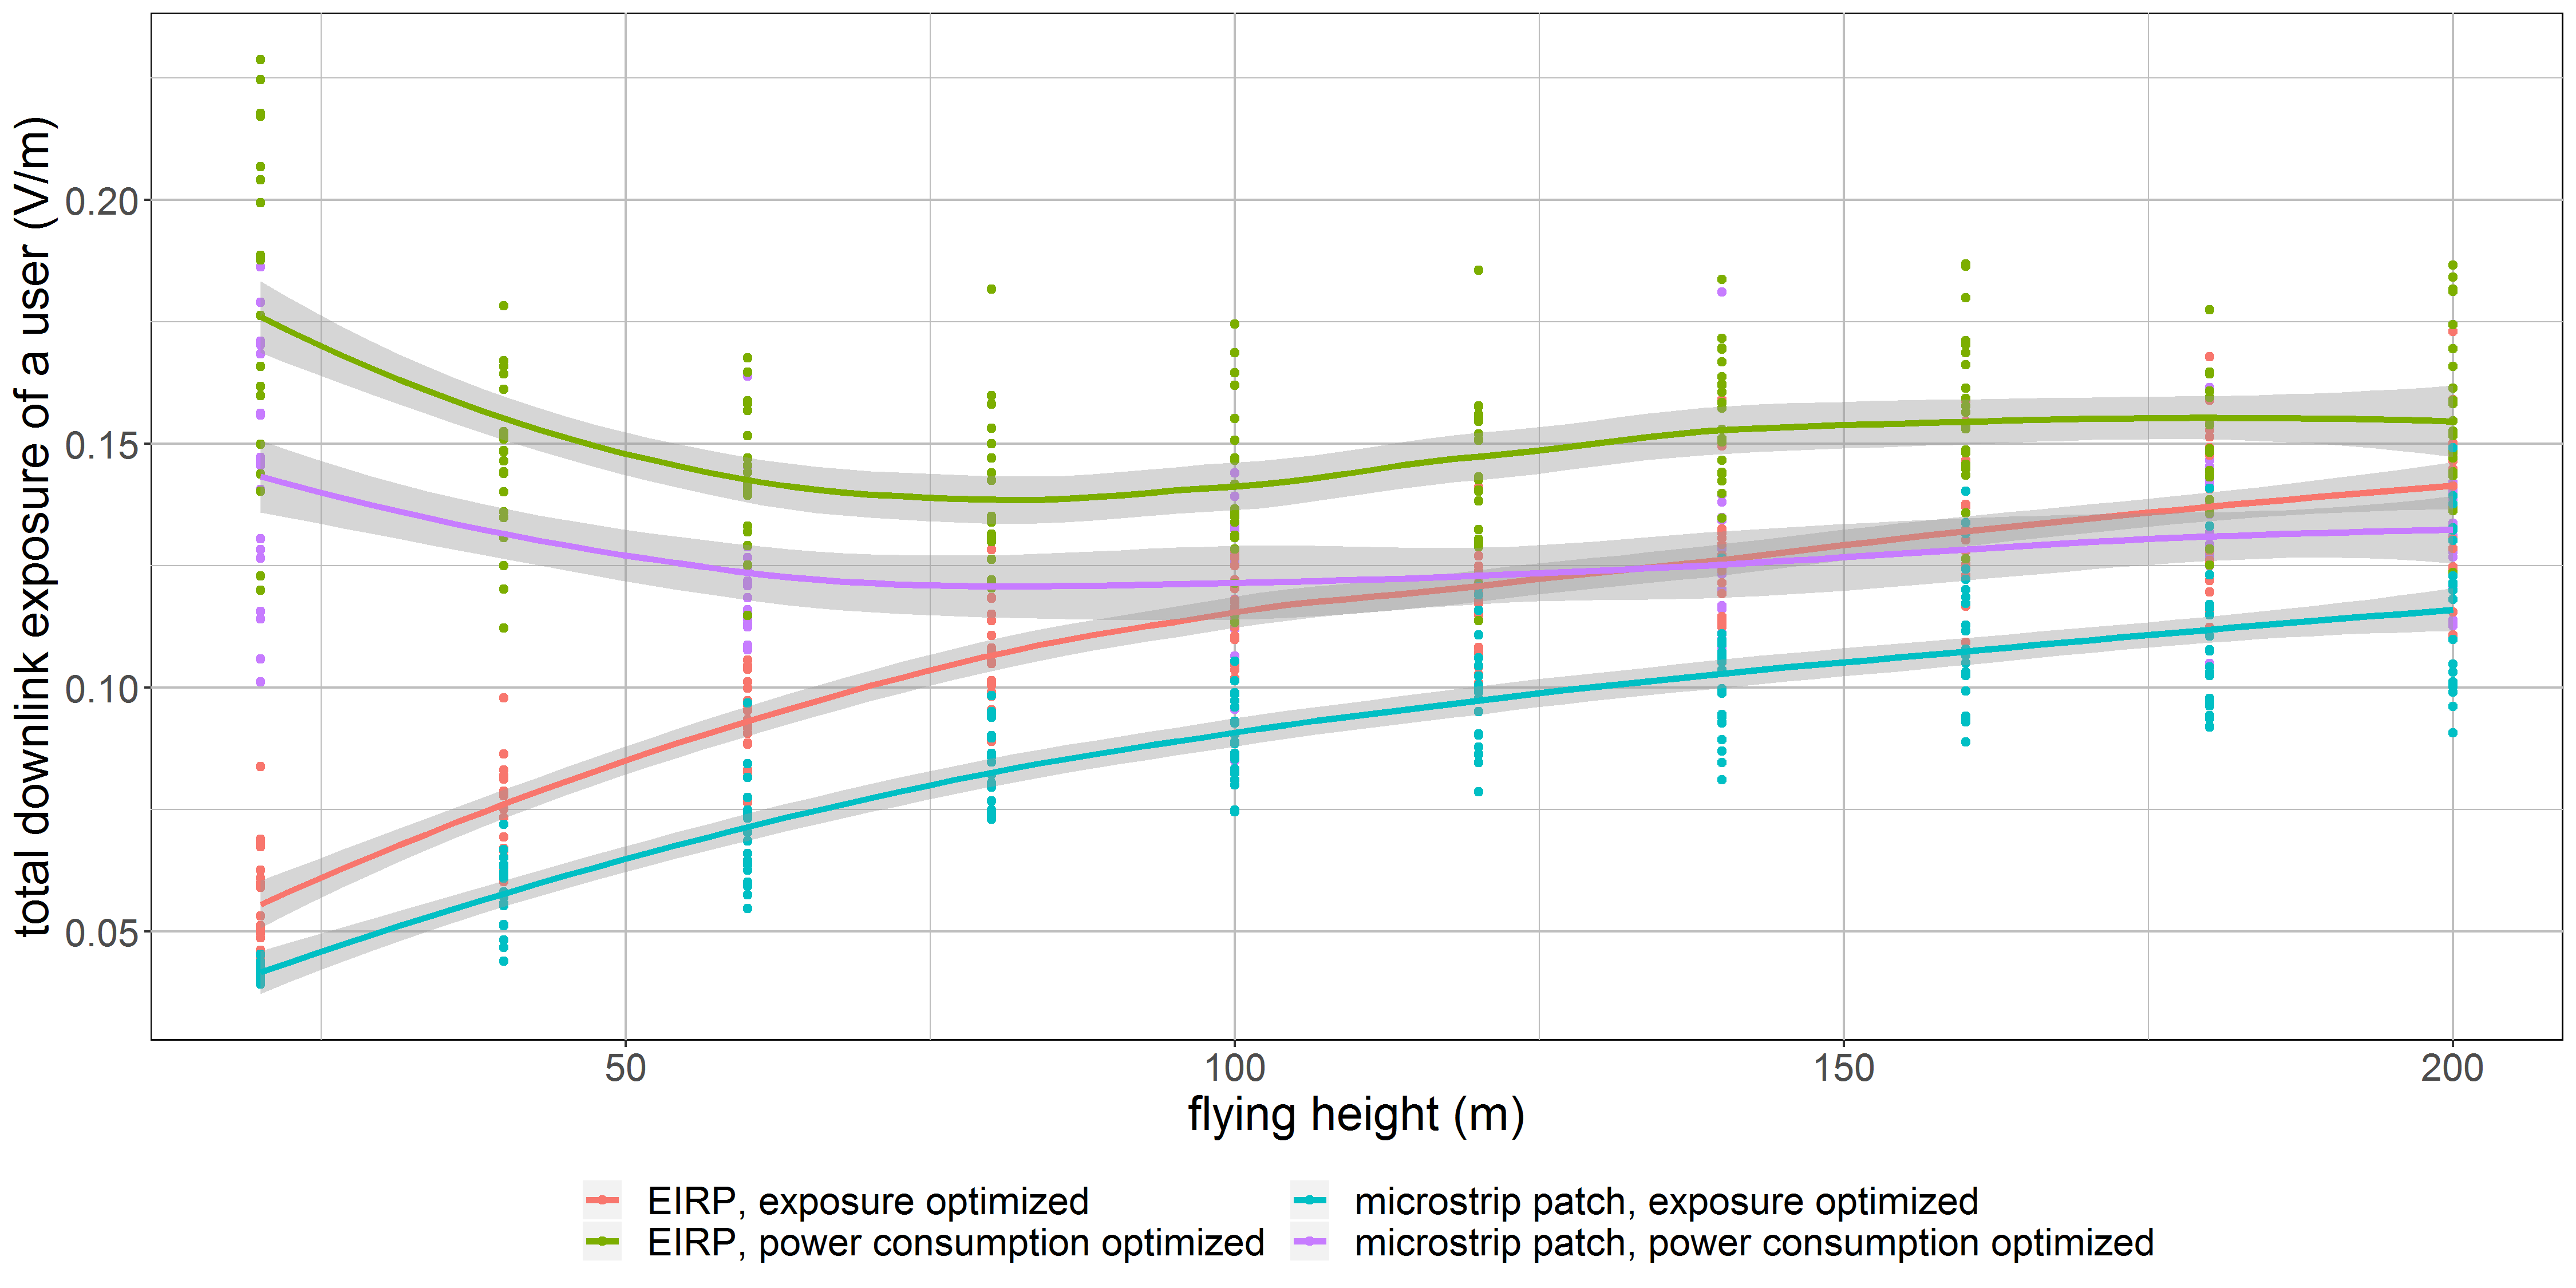
\includegraphics[width=\textwidth]{../results/s3/fhvsdl.png}
  \caption{The influence of the flying height on the downlink electromagnetic radiation of the average user.}
  \label{fig:s3fhvsdl}
\end{figure}

\begin{figure}[]
  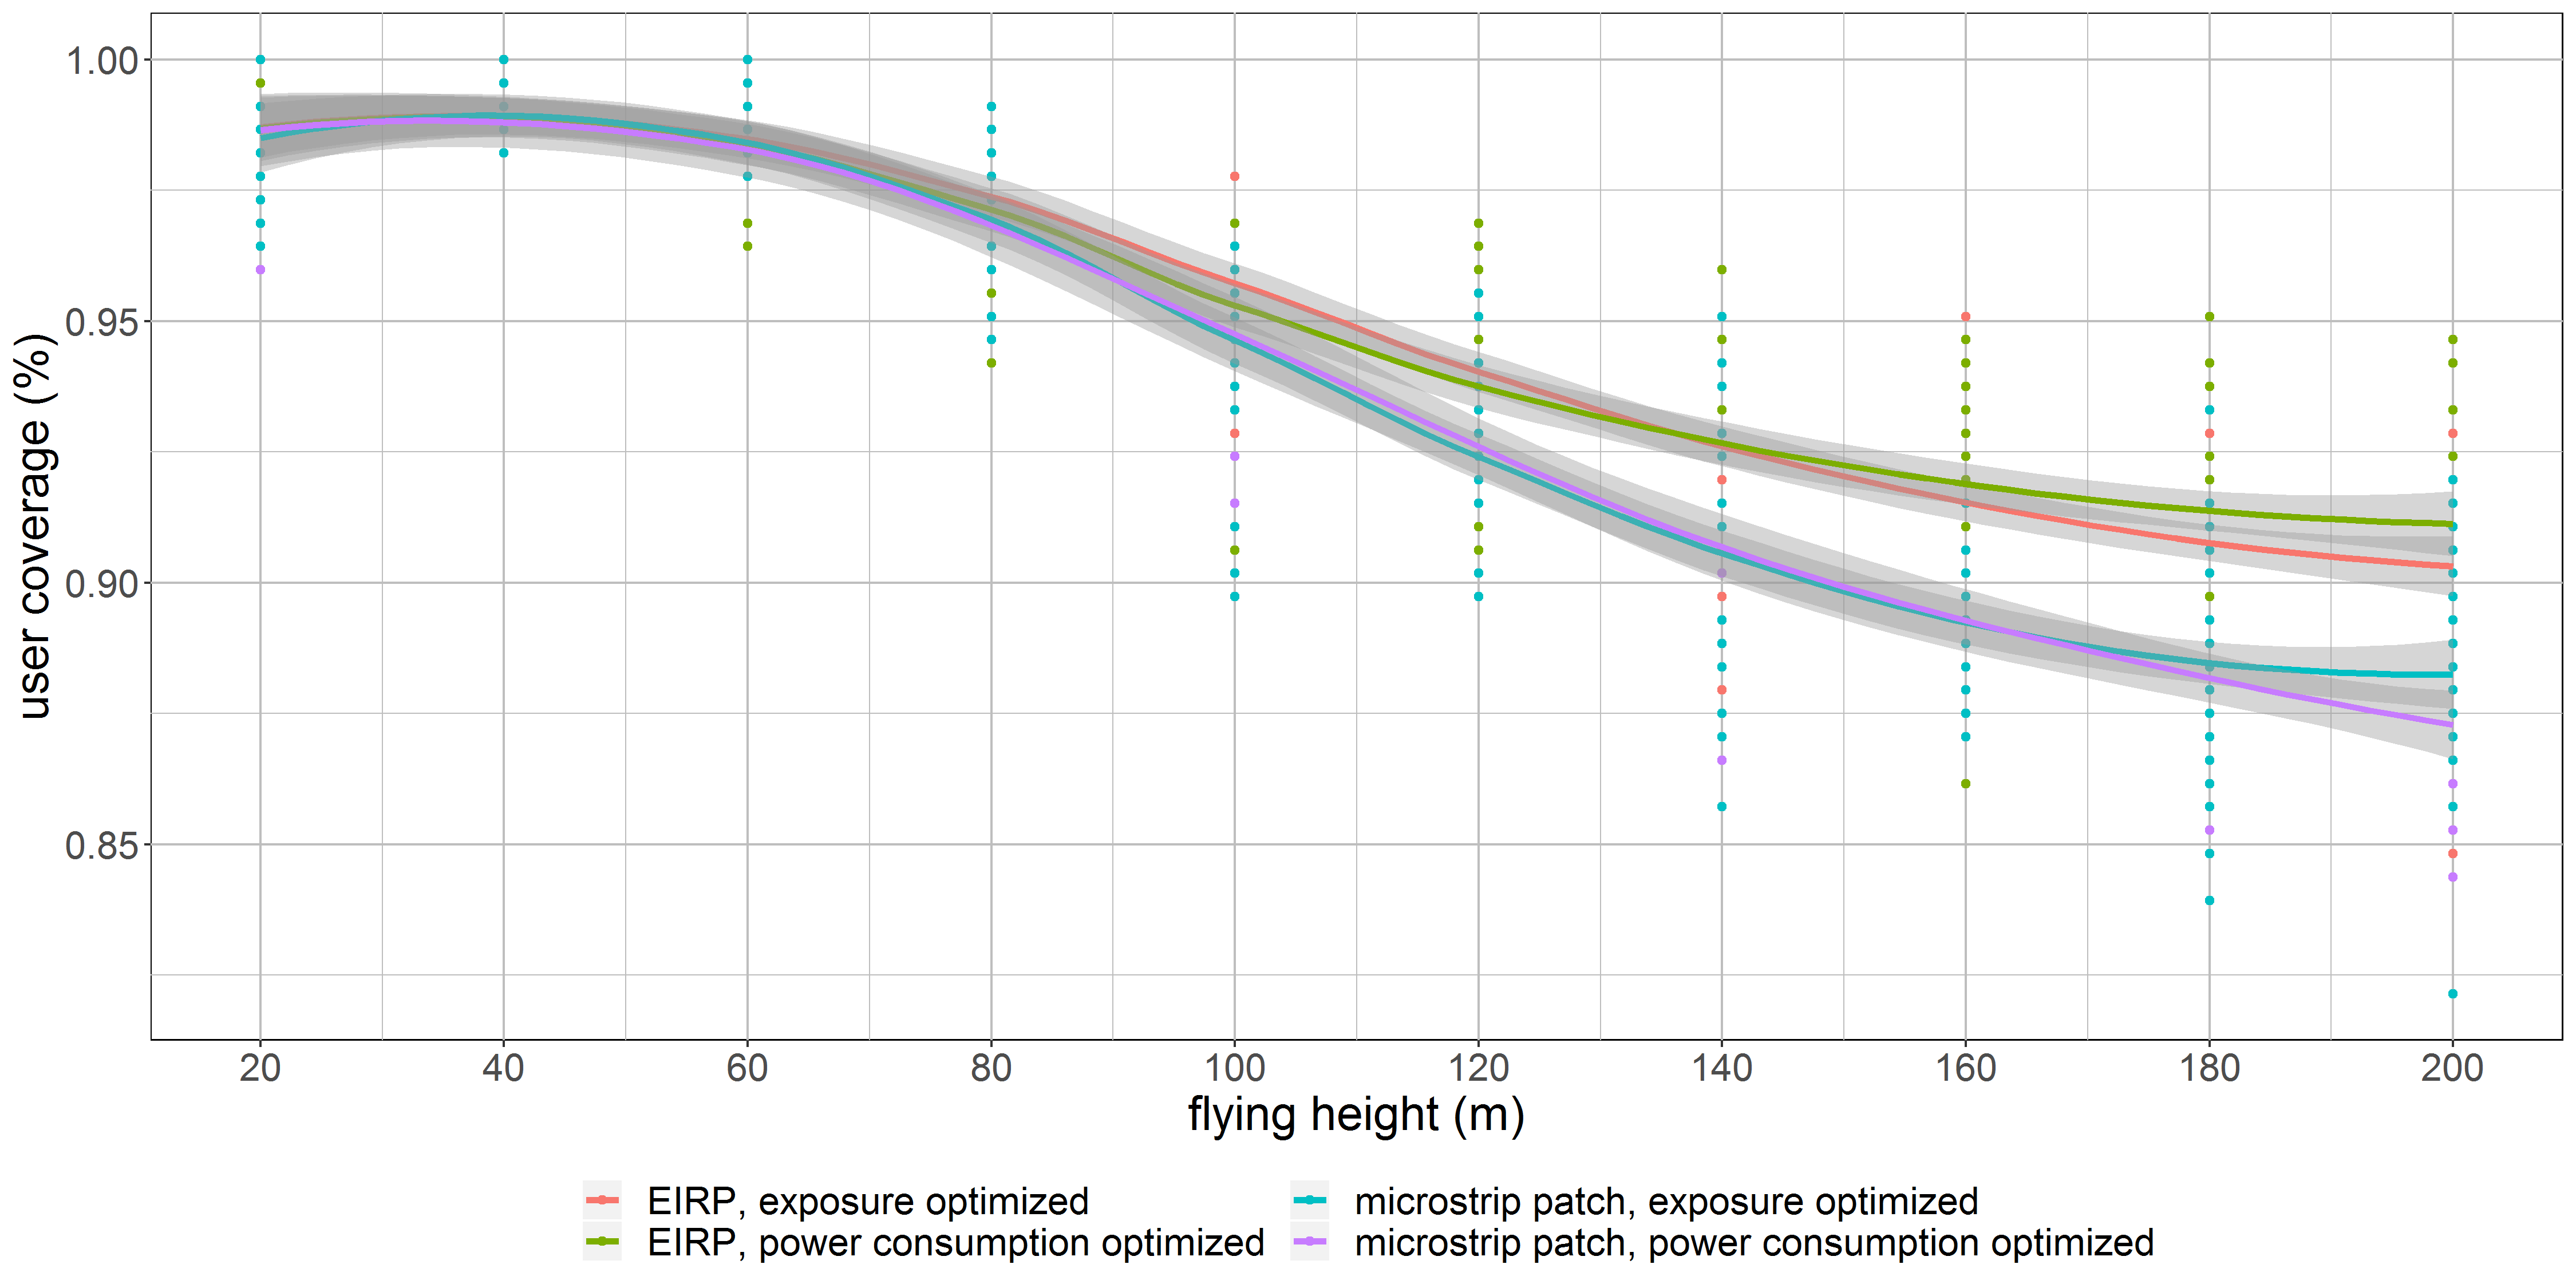
\includegraphics[width=\textwidth]{../results/s3/fhvscov.png}
  \caption{This graph shows the percentage of covered users by one drone for different flying heights.}
  \label{fig:s3fhvscov}
\end{figure}

\begin{figure}[]
  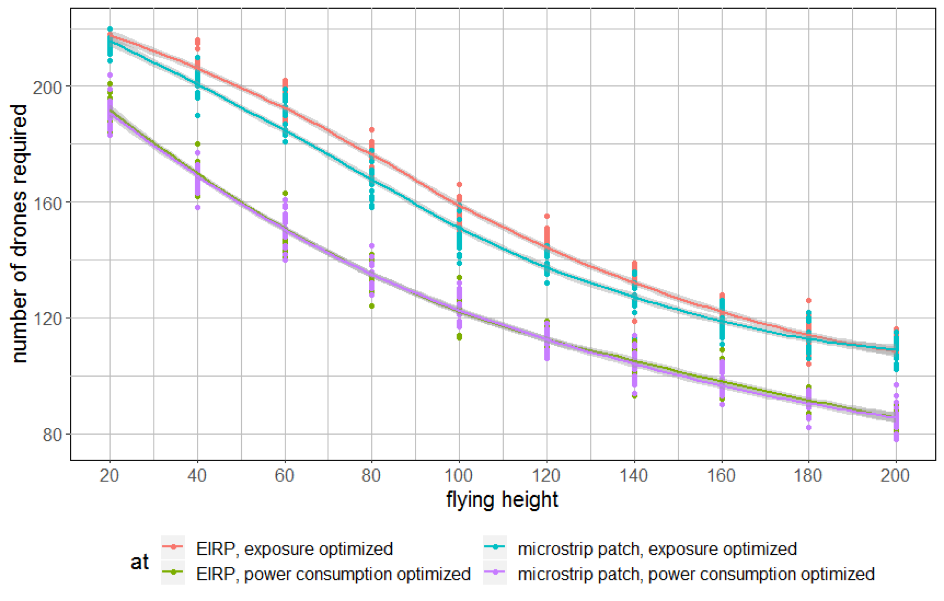
\includegraphics[width=\textwidth]{../results/s3/fhvsnumdrones.png}
  \caption{This graph shows how much drones are required for different flying heights while trying to achieve a 100\% coverage.}
  \label{fig:s3fhvscov}
\end{figure}

\begin{figure}[h!]
  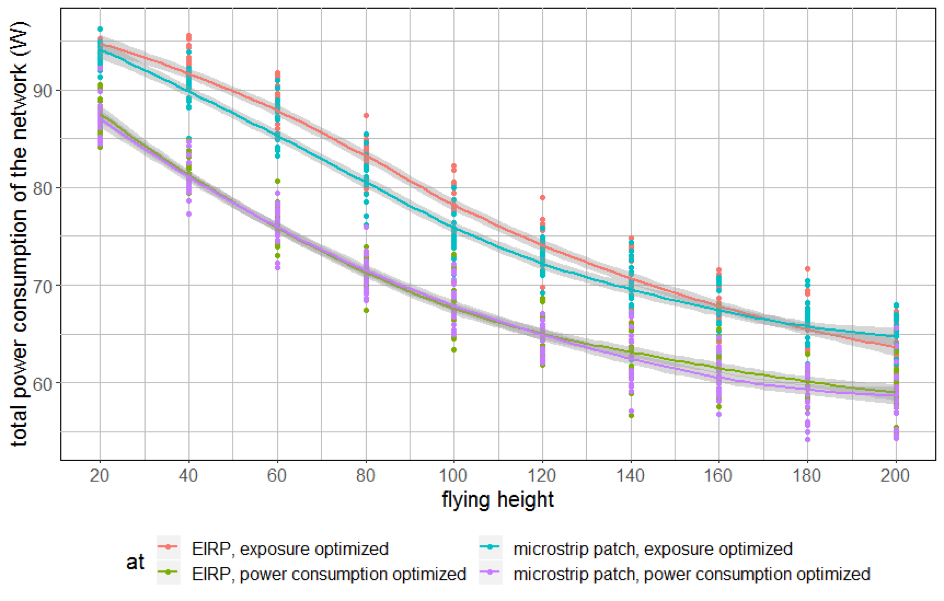
\includegraphics[width=\textwidth]{../results/s3/fhvspc.png}
  \caption{The influence of the flying height on the total power consumption of the network.}
  \label{fig:s3fhvspc}
\end{figure}

Both \ref{fig:s3fhvsnumdrones} and \ref{fig:s3fhvspc} show that the network profit from increasing the flying altitude. 
Not only less drones are needed but also the power consumption is lower. Both can be explained by the lower pathloss when \gls{UABS}s fly higher.
If a user cannot be covered because an \gls{UABS}s is too far away or is saturated with other users, 
the tool can simply add another \gls{UABS}. The only remaining reason that a user can’t be covered is because the position of 
the drone is obstructed by a building. The higher drones fly, the less change the position is obstructed by a building. 
In gent is this chance is zero when flying higher then 119 meters. Since the `Artevelde Tower' is the highest building in Ghent.

Scenario 1 already proved that with low flying drones, the main source of electromagnetic radiation are \gls{UABS}. 
This changes around 80 meters where \gls{UL} electromagnetic radiation of the \gls{UE}
 exceeds \gls{DL} radiation in order to still be able to reach the high flying \gls{UABS}s.

\begin{figure}[]
  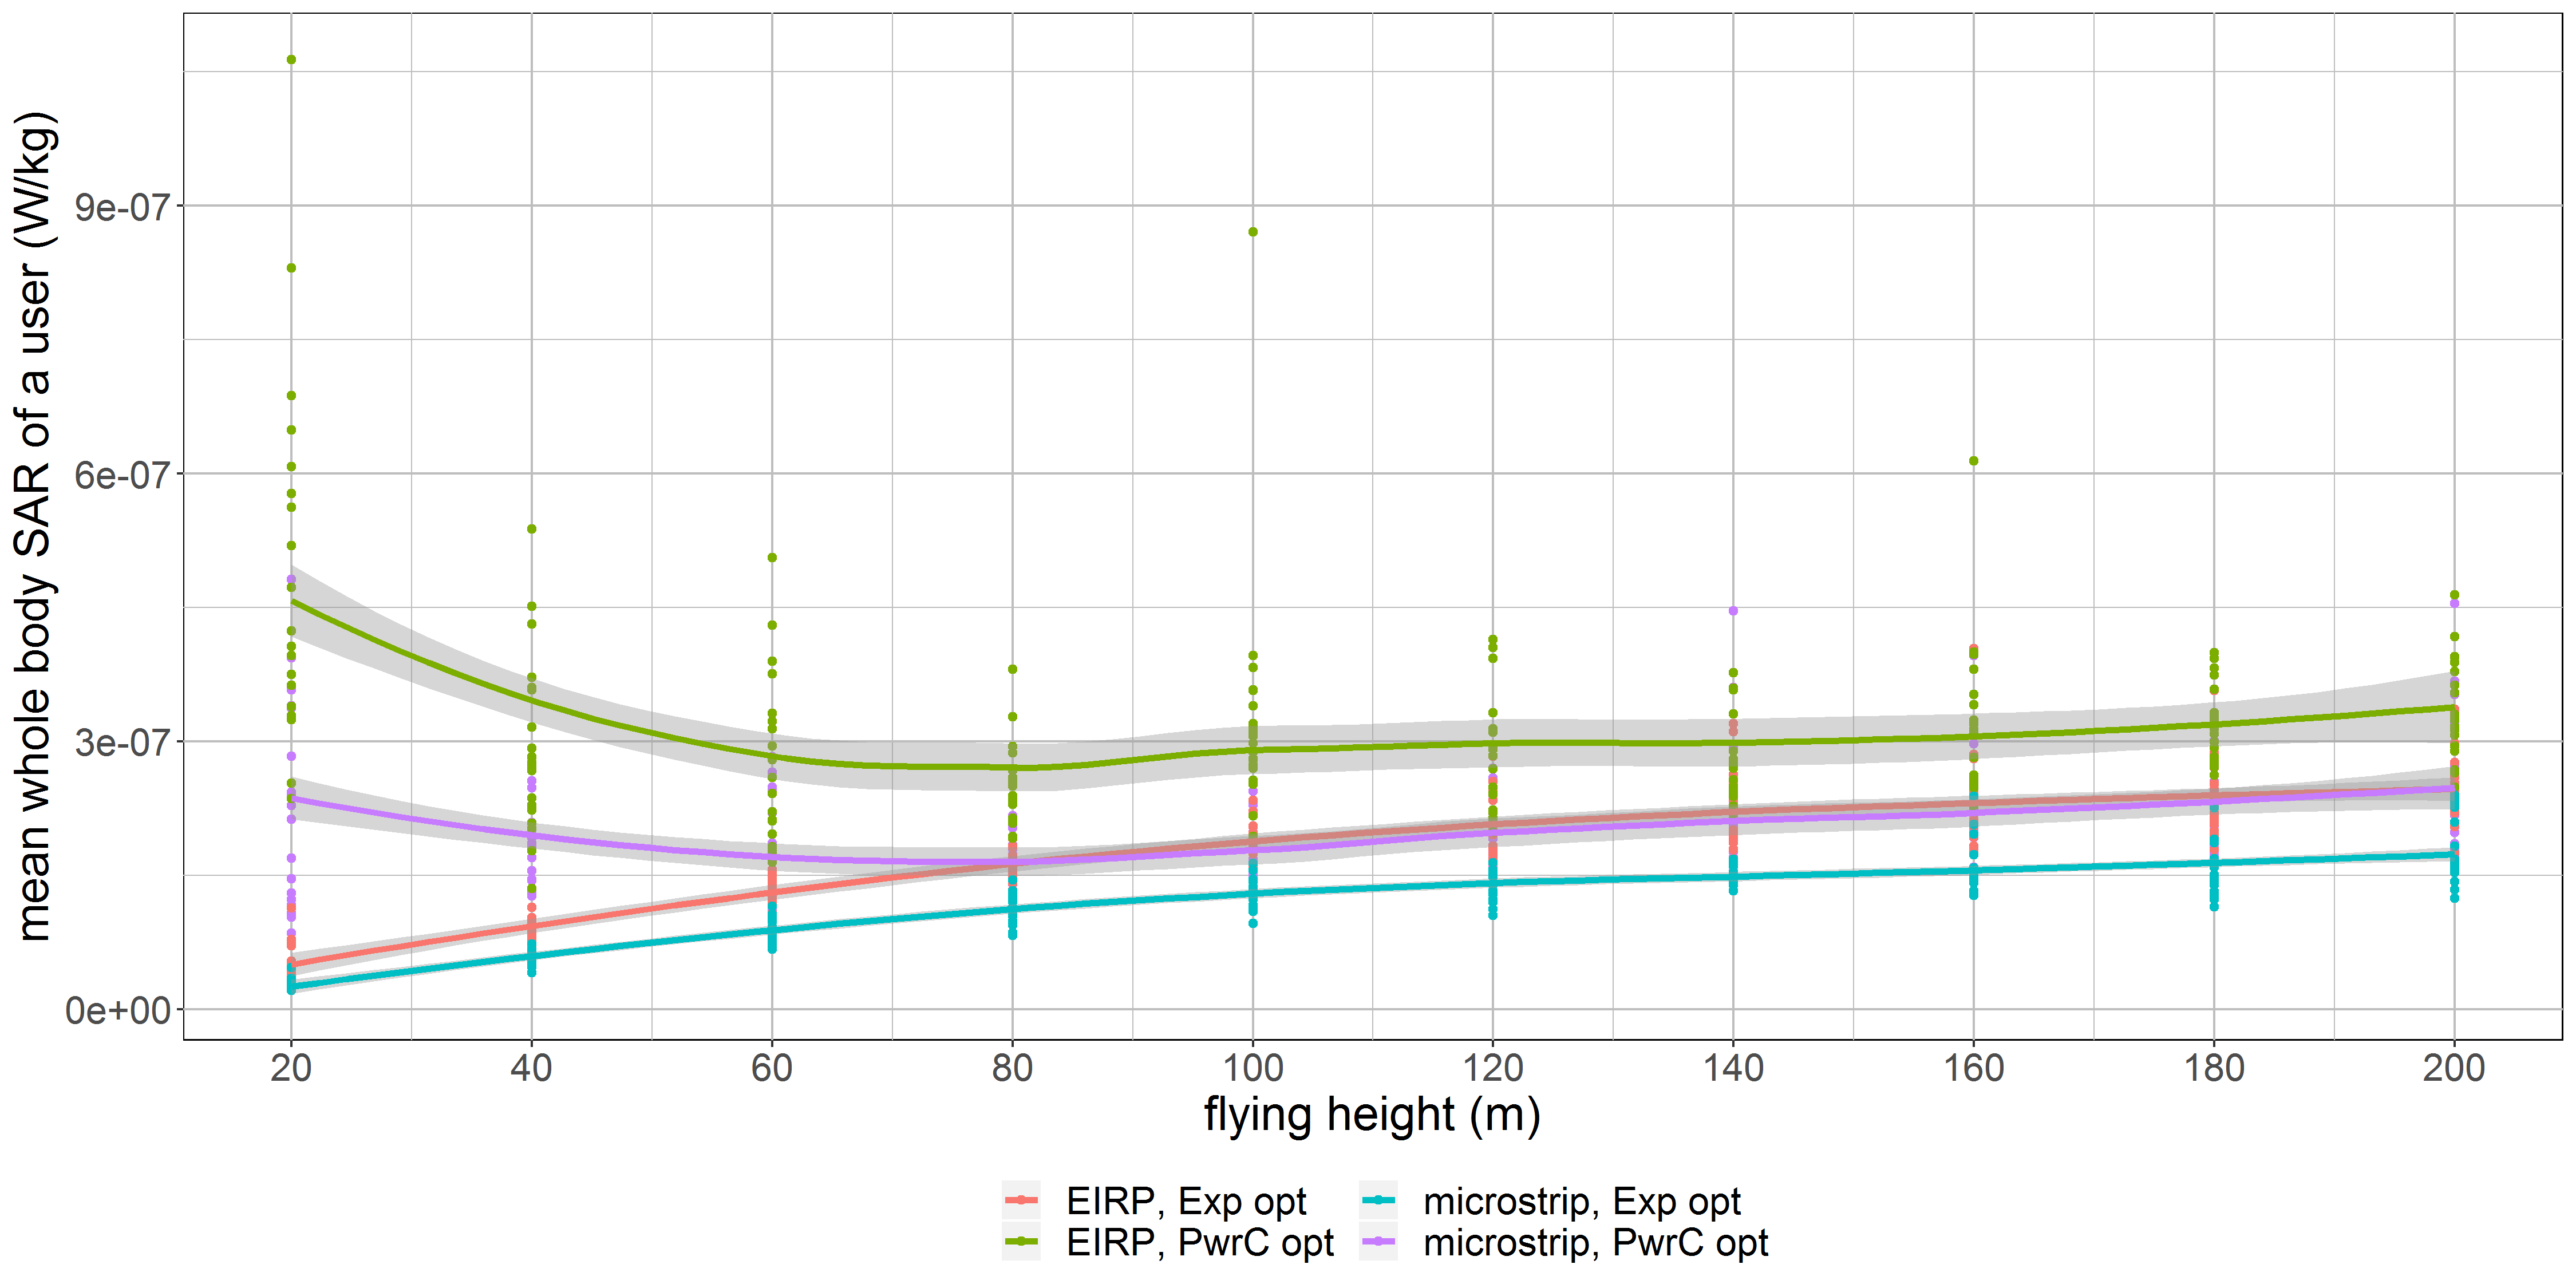
\includegraphics[width=\textwidth]{../results/s3/fhvssar.png}
  \caption{The influence of the flying height on the weighted average $SAR_{10g}$ of users in the network.}
  \label{fig:s3fhvssar}
\end{figure}

\subsection{Influence of the number of users}
todo